

%%%%%%%%%%%%%%%%%%%%%%%%%%%%%%%%%%%%%%%%%%%%%%%%%%%%%%%%%%%%%%%%%%%%%%%%%%%%%%%%
% Thesis / Project Report
% LaTeX Template
% Version 2.0 (08/04/16)
%
% Author:
% Parth Ganeriwala
% https://github.com/ParthGaneriwala/BITS-Thesis-Template-Latex
%
% This template is heavily based on the work of Siddhant Shrivastava, Darshit Shah, Steven Gunn and Sunil Patel
% Siddhant Shrivastava
% https://github.com/sidcode/bits-pilani-thesis-template-latex
% Darshit Shah
% https://github.com/darnir/BPHC-LaTeX-Report-Class
% Steven Gunn
% http://users.ecs.soton.ac.uk/srg/softwaretools/document/templates/
% and
% Sunil Patel
% http://www.sunilpatel.co.uk/thesis-template/
%
% License:
% CC BY-NC-SA 4.0 (http://creativecommons.org/licenses/by-nc-sa/4.0/)
%
% Note:
% Make sure to edit document variables in the Thesis.cls file
%
%%%%%%%%%%%%%%%%%%%%%%%%%%%%%%%%%%%%%%%%%%%%%%%%%%%%%%%%%%%%%%%%%%%%%%%%%%%%%%%%

%-------------------------------------------------------------------------------
%	PACKAGES AND OTHER DOCUMENT CONFIGURATIONS
%-------------------------------------------------------------------------------

\documentclass[11pt, a4paper, oneside, british]{Thesis}
% \includeonly{Appendices/Appendix-A} % Paper size, default font size
                                               % and one-sided paper

\graphicspath{{Figures}} % Specifies the directory where pictures are stored

\usepackage[sorting=none,bibstyle=numeric-comp,citestyle=numeric,backend=bibtex,defernumbers=true]{biblatex}  
\addbibresource{References.bib} % Specifies the bibliography file to be used 
\usepackage{physics}  
\usepackage{float} 
\usepackage{bookmark}  
\usepackage{multirow}  
\usepackage{booktabs, makecell}  
\usepackage[table, svgnames]{xcolor}  
\usepackage{siunitx}  
\usepackage{colortbl}  
\usepackage{wrapfig}  
\usepackage{bbm}  
\usepackage{ragged2e}  
\usepackage{array}  
\usepackage{scalerel}  
\usepackage{hyperref}  
\usepackage{mdframed}
\usepackage{tcolorbox}
\usepackage{bbold}
\usepackage{mhchem}
\usepackage{booktabs}
\definecolor{Gray}{gray}{0.9}  
\newlength\mysep   
\setlength\mysep{1cm}  
\DeclareFloatSeparators{mysep}{\hskip\mysep}  

\AtBeginDocument{\RenewCommandCopy\qty\SI}  
\ExplSyntaxOn  
\msg_redirect_name:nnn { siunitx } { physics-pkg } { none }  
\ExplSyntaxOff  

\title{\ttitle}
\makeatletter  
\pdfstringdefDisableCommands{\let\HyPsd@CatcodeWarning\@gobble}  
\makeatother  

\usepackage[T1]{fontenc}
\begin{document}

\frontmatter % Use roman numbering style (i, ii...) for the pre-content pages

\setstretch{1.3} % Line spacing of 1.3

% Define page headers using FancyHdr package and set up for one-sided printing
\fancyhead{} % Clears all page headers and footers
\rhead{\thepage} % Sets the right side header to show the page number
\lhead{} % Clears the left side page header

\pagestyle{fancy} % Finally, use the "fancy" page style to implement the
                  %FancyHdr headers

% Input all the variables used in the document. Please fill out the
% variables.tex file with all your details.
%-------------------------------------------------------------------------------
%	DOCUMENT VARIABLES
%
%	Fill in the lines below to set the various variables for the document
%-------------------------------------------------------------------------------

%-------------------------------------------------------------------------------
% Your thesis title - this is used in the title and abstract
% Command: \ttitle
\thesistitle{Bachelor Thesis}
%-------------------------------------------------------------------------------
% The document type: Thesis / report, etc.
% Command: \doctype
\documenttype{Undergraduate Thesis}
%-------------------------------------------------------------------------------
% Your supervisor's name - this is used in the title page
% Command: \supname
\supervisor{Henry \textsc{Pinto}}
%-------------------------------------------------------------------------------
% The supervisor's position - Used on Certificate
% Command: \suppos
\supervisorposition{Associate PhD Professor}
%-------------------------------------------------------------------------------
% Supervisor's institute
% Command: \supinst
\supervisorinstitute{Yachay Tech University}
\supervisorinstitutecountry{Urcuqui, Ecuador}
%-------------------------------------------------------------------------------
% Your Co-Supervisor's name
% Command: \cosupname
\cosupervisor{Andres \textsc{Garay}}
%-------------------------------------------------------------------------------
% Co-Supervisor's Position - Used on Certificate
% Command: \cosuppos
\cosupervisorposition{Associate PhD Professor}
%-------------------------------------------------------------------------------
% Co-Supervisor's Institute
% Command: \cosupinst
\cosupervisorinstitute{Centro de Investigacion en Materiales Avanzados}
\cosupervisorinstitutecountry{Monterrey, Mexico}
%-------------------------------------------------------------------------------
% Your Examiner's name. Not currently used anywhere.
% Command: \examname
\examiner{}
%-------------------------------------------------------------------------------
% Name of your degree
% Command: \degreename
\degree{Bachelor of Physics}
%-------------------------------------------------------------------------------
% The BITS Course Code for which this report is written
% COmmand: \ccode
\coursecode{BITS F421T}
%-------------------------------------------------------------------------------
% The name of the Course
% Command: \cname
\coursename{Thesis}
%-------------------------------------------------------------------------------
% Your name. Extend manually in case of multiple authors
% Command: \authornames
\authors{J. Gabriel \textsc{Balarezo}}
%-------------------------------------------------------------------------------
% Your ID Number - used on the Title page and abstract
% Command: \idnum
\IDNumber{0106019219}
%-------------------------------------------------------------------------------
% Your address
% Command: \addressnames
\addresses{}
%-------------------------------------------------------------------------------
% Your subject area
% Command: \subjectname
\subject{}
%-------------------------------------------------------------------------------
% Keywords for this report.
% Command: \keywordnames
\keywords{Ab initio calculations, electronic properties, magnetic properties, XGeTe$_3$ monolayers, VASP, PBE,PBESol, Phonopy, Alloy-Theoretic Automated Toolkit, Hubbard U corrections.}
%-------------------------------------------------------------------------------
% University details
% Command: \univname
\university{\texorpdfstring{\href{https://www.bits-pilani.ac.in/Dubai/index.aspx} % URL
                {Yachay Tech University}} % University name
                {Yachay Tech University}}
%-------------------------------------------------------------------------------
% University details, in Capitals
% Command: \UNIVNAME
\UNIVERSITY{\texorpdfstring{\href{https://www.bits-pilani.ac.in/Dubai/index.aspx} % URL
                {Yachay Tech University}} % name in capitals
                {Yachay Tech University}}
                
\UNIVERSITYCOUNTRY{\texorpdfstring{Urcuqui, Ecuador}}
%-------------------------------------------------------------------------------
% Department Details
% Command: \deptname
%\department{\texorpdfstring{\href{https://www.bits-pilani.ac.in/dubai/computerscience/DetofComputerScience} % Your department's URL
%                {Computer Science}} % Your department's name
%                {Computer Science}}
%-------------------------------------------------------------------------------
% Department details, in Capitals
% Command: \DEPTNAME
%\DEPARTMENT{\texorpdfstring{\href{https://www.bits-pilani.ac.in/dubai/computerscience/DetofComputerScience} % Your department's URL
%                {Computer Science}} % Your department's name in capitals
%                {Computer Science}}
%-------------------------------------------------------------------------------
% Research Group Details
% Command: \groupname
\group{\texorpdfstring{\href{Research Group Web Site URL Here (include http://)}
                {Research Group Name}} % Your research group's name
                {Research Group Name}}
%-------------------------------------------------------------------------------
% Research Group Details, in Capitals
% Command: \GROUPNAME
\GROUP{\texorpdfstring{\href{Research Group Web Site URL Here (include http://)}
                {RESEARCH GROUP NAME (IN BLOCK CAPITALS)}}
                {RESEARCH GROUP NAME (IN BLOCK CAPITALS)}}
%-------------------------------------------------------------------------------
% Faculty details
% Command: \facname
\faculty{\texorpdfstring{\href{Faculty Web Site URL Here (include http://www.yachaytech.edu.ec/en/physicsandnanotech/)}
                {School of Physical Sciences and Nanotechnology}}
                {School of Physical Sciences and Nanotechnology}}
%-------------------------------------------------------------------------------
% Faculty details, in Capitals
% Command: \FACNAME
\FACULTY{\texorpdfstring{\href{Faculty Web Site URL Here (include http://)}
                {FACULTY NAME (IN BLOCK CAPITALS)}}
                {FACULTY NAME (IN BLOCK CAPITALS)}}
%-------------------------------------------------------------------------------


%-------------------------------------------------------------------------------
%   NON-CONTENT PAGES
%-------------------------------------------------------------------------------
\maketitle

\Authorship

\Declaration

\Dedicatory{
To the younger self who dared to begin, \\
and to the present self who refused to stop. \\
For every sleepless night and every \\
quiet triumph along the way.
} 
%\Acknowledgements

\Resumen

\Abstract



% \Quotation{Insert Random Quote here. Publish like a boss.}{Your Name}





%-------------------------------------------------------------------------------
%	LIST OF CONTENTS/FIGURES/TABLES PAGES
%-------------------------------------------------------------------------------

% The page style headers have been "empty" all this time, now use the "fancy"
% headers as defined before to bring them back
\pagestyle{fancy}

\lhead{\emph{Contents}} % Set the left side page header to "Contents"
\tableofcontents % Write out the Table of Contents

% Set the left side page header to "List of Figures"
\lhead{\emph{List of Figures}}
\listoffigures % Write out the List of Figures

 % Set the left side page header to "List of Tables"
\lhead{\emph{List of Tables}}
\listoftables % Write out the List of Tables

%-------------------------------------------------------------------------------
%	ABBREVIATIONS
%-------------------------------------------------------------------------------


%-------------------------------------------------------------------------------
%	PHYSICAL CONSTANTS/OTHER DEFINITIONS
%-------------------------------------------------------------------------------

% \clearpage % Start a new page

% % Set the left side page header to "Physical Constants"
% \lhead{\emph{Physical Constants}}

%  % Include a list of Physical Constants (a four column table)
% \listofconstants{lrcl}
% {
% Speed of Light & $c$ & $=$ & $2.997\ 924\ 58\times10^{8}\ \mbox{ms}^{-\mbox{s}}$ (exact)\\
% % Constant Name & Symbol & = & Constant Value (with units) \\
% }

%-------------------------------------------------------------------------------
%	SYMBOLS
%-------------------------------------------------------------------------------

% \clearpage % Start a new page

% \lhead{\emph{Glossary}} % Set the left side page header to "Symbols"

% \listofnomenclature % List the nomenclature. (We use the glossaries package)

%-------------------------------------------------------------------------------
%	DEDICATION
%-------------------------------------------------------------------------------

\mainmatter % Begin numeric (1,2,3...) page numbering

\pagestyle{fancy} % Return the page headers back to the "fancy" style

% Include the chapters of the thesis as separate files from the Chapters folder
% Uncomment the lines as you write the chapters

% Chapter Template

\chapter{Introduction} % Main chapter title

\label{Chapter1} % Change X to a consecutive number; for referencing this chapter elsewhere, use \ref{ChapterX}

\lhead{Chapter 1. \emph{Introduction}} % Change X to a consecutive number; this is for the header on each page - perhaps a shortened title

%----------------------------------------------------------------------------------------
%	SECTION 1
%----------------------------------------------------------------------------------------

%############################# Introduction #################################
\section{Background}
Concrete is the synthetic material currently produced in volumes larger than any other material on Earth. With an annual consumption of approximately 35 billion metric tonnes, it is only second to water in terms of global usage \cite{mehta2014concrete, Monteiro2017}. It plays a pivotal role in the construction industry, serving as the backbone for buildings, roads, bridges, dams, and many other infrastructure elements central to modern society. Its widespread adoption is the result of its unique combination of properties, including high compressive strength, durability, versatility, and cost-effectiveness \cite{mehta2014concrete}, rendering it an important asset that directly influences the quality of life and economic development worldwide \cite{VanDamme2018, Biernacki2017}. Nevertheless, the massive production and use of concrete come with significant environmental challenges. The production of its main constituent, Portland cement, is responsible for 8-9\% of the global anthropogenic CO$_2$ emissions \cite{Monteiro2017}. Additionally, around 40\% of produced concrete is employed to repair and maintain existing infrastructure \cite{mehta2014concrete}, which aggravates the environmental impact of concrete. Therefore, the development of more durable and sustainable concrete is of utmost importance, which requires a better understanding of concrete's composition and microstructure. 

Concrete itself is a composite material and can be regarded as a two-phase system \cite{mehta2014concrete}---the aggregate phase, composed of particles of varying size and shape; and the binding medium, composed of hydrated cement paste. The latter is, in turn, a heterogeneous mixture of different cement hydration products, with calcium silicate hydrate (C--S--H)\footnote{
Conventional cement chemistry notation: C = CaO, S = SiO$_2$, H = H$_2$O
} being the most abundant and important phase. C--S--H makes up 50 to 60\% of the volume of solids in a hydrated cement paste and is responsible for the majority of the long-term strength and durability of concrete \cite{mehta2014concrete}. Together, the aggregate and binding phases form a complex microstructure that bridges the nanoscale chemistry of hydration products with the properties of concrete at the engineering scale. Nonetheless, the underlying microstructure-property relationships in concrete are not yet fully understood, hindering our ability to manipulate and tailor its properties for specific applications. 


In this context, numerous efforts have been made to understand and model the properties of C--S--H, owing to its central role in determining the properties of concrete \cite{Ji2012, Papatzani2015, Qomi2020}. Characterisation techniques---such as X-ray diffraction (XRD) \cite{Allen2007, Houston2009, Oh2012}, nuclear magnetic resonance (NMR) \cite{Foley2012, Maddalena2019}, and small angle neutron scattering (SANS)---have provided valuable insights into the structure and composition of C--S--H upon which many molecular models have been developed. The pioneering work of Pellenq \emph{et al.} \cite{Pellenq2009}---which introduced a realistic molecular model of cement hydrates---paved the way for a wide range of molecular modelling techniques \cite{AbdolhosseiniQomi2014, Richardson2014, Bauchy2014, Kovacevic2016, KunhiMohamed2018} intended to capture the nanoscale structure and properties of C--S--H accurately. Additionally, the advancement of computational power and the development of efficient molecular dynamics (MD) simulation methods have enabled the exploration of mechanical, thermal, and transport properties of C--S--H \cite{
AbdolhosseiniQomi2015, Bahraq2022, Cho2020, Barbhuiya2023} under conditions that are relevant to concrete applications but difficult to replicate experimentally. The upscaling of C--S--H properties can be viewed from a hierarchical multiscale perspective, as illustrated in Figure \ref{fig:figure1}, which highlights the microstructure-property relationships of C--S--H at different scales and the relevance of nanoscale properties to the engineering scale of concrete.
\begin{figure}[H]
    \centering
    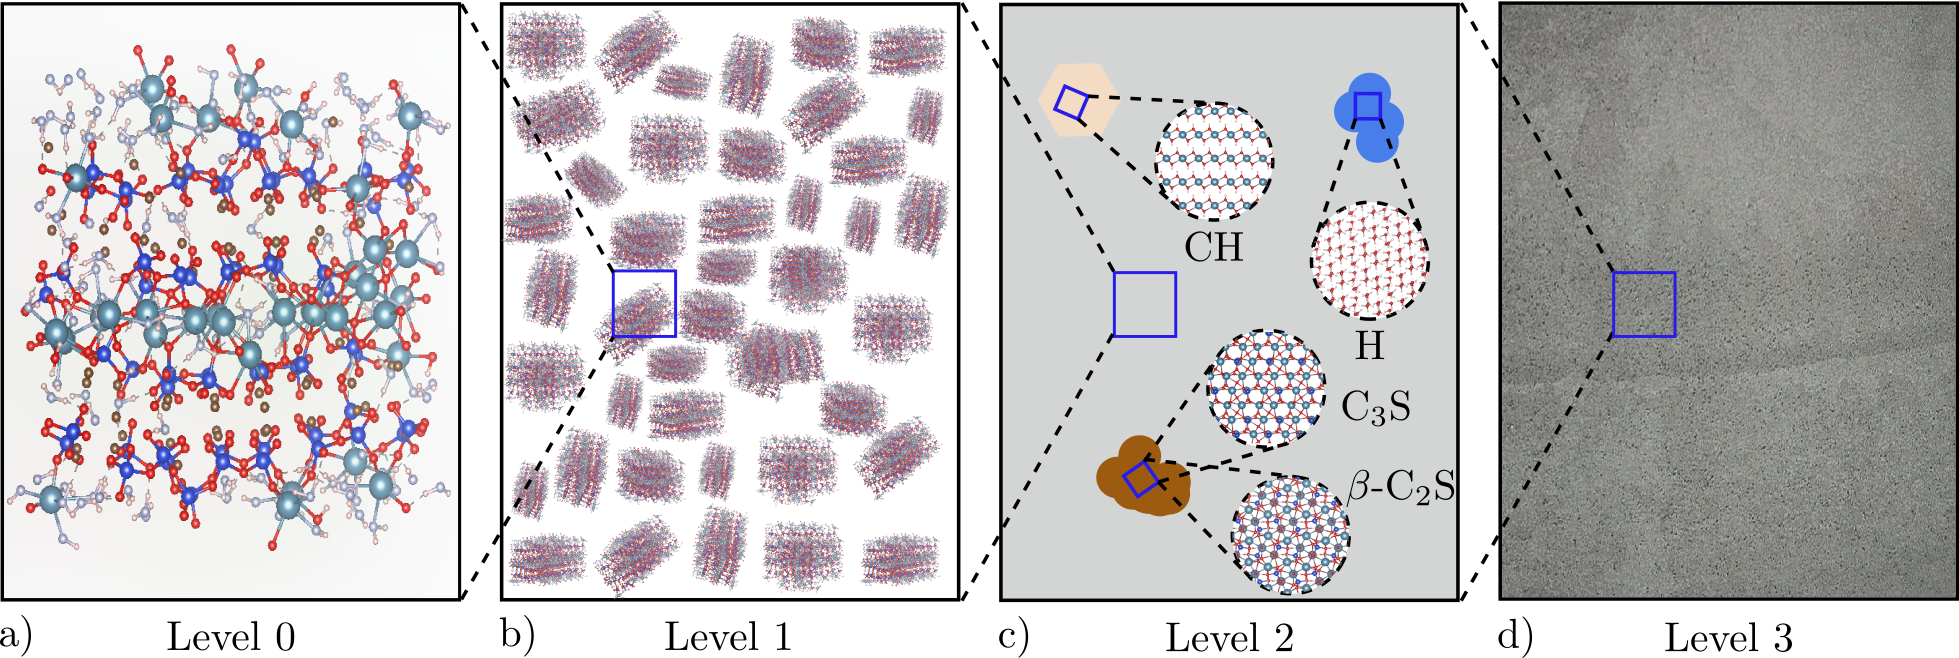
\includegraphics[width=0.9\textwidth]{levels.png}
    \caption{A four-level model representing the upscaling of C--S--H properties from the nanoscale to the engineering scale. (a) snapshot of C--S--H's nanostructure. (b) microstructure of C--S--H created by agglomeration of randomly oriented C--S--H nanoparticles. (c) microtexture of hardened paste composed of hydration products. (d) Macrotexture of cement paste at the engineering scale. Adapted from Ref. \cite{AbdolhosseiniQomi2015}.}
    \label{fig:figure1}
\end{figure}

Despite the significant progress made in understanding C--S--H at the atomic scale, the inherent complexity of this material makes it challenging to model its structure and properties using classical methods realistically ---primarily molecular dynamics (MD) simulations. Resorting to \emph{ab initio} methods---such as density functional theory (DFT)---can hugely improve the accuracy of these models, but demand high computational resources, making it nearly intractable for real applications \cite{zotero-item-16}. In this context, machine learning (ML) based concrete research has emerged as a promising approach to address these challenges \cite{zotero-item-16, Kobayashi2021, Zhu2024}. Trained on large, high-quality \emph{ab initio} datasets, ML models can capture the underlying physics of C--S--H and predict its properties with high accuracy, comparable to that of first-principles methods, while requiring significantly less computational power. 

%-----------------------------------
%	SUBSECTION 1
%-----------------------------------
\section{Problem Statement}
Concrete production is projected to increase by 50\% annually by 2050 \cite{Monteiro2017}, and with no foreseeable alternatives to Portland cement, the urgent need for more sustainable concrete is evident. The development of advanced concrete with enhanced durability and performance could significantly lower the environmental burden. State-of-the-art methods such as machine learning show great potential to accelerate this transition, providing a powerful tool to advance our understanding of concrete's microstructure and properties. 

In this regard, this report aims to investigate the performance of a machine learning force field (MLFF) in modelling and predicting the mechanical properties of C--S--H. Such MLFF will be trained and validated
using \emph{ab initio} data, ensuring it captures the complex atomic interactions and structural variability of C--S--H. Ultimately, our goal is to develop a reliable and computationally efficient model that can predict the mechanical properties of C--S--H, thereby supporting concrete research towards a sustainable future.
%-----------------------------------
%	SUBSECTION 2
%-----------------------------------

\section{General and Specific Objectives}
The main goal of this work is to use density functional theory (DFT), \emph{ab initio} molecular dynamics (AIMD), and machine learning (ML) to
develop a machine learning force field (MLFF) for calcium silicate hydrates (C--S--H) to study the mechanical properties of C--S--H. To achieve this, the following specific objectives are defined:
\begin{itemize}
    \item To describe the theoretical foundations of DFT, AIMD, and MLFFs, including key concepts on exchange-correlation functionals such as PBE and PBEsol, and pseudopotentials. 
    \item To perform geometric relaxation on bulk C--S--H model employing the VASP software with the PBEsol functional.
    \item To analyse the electronic structure of C--S--H by computing the density of states (DOS) of C--S--H.
    \item To train, refit, and test an MLFF using AIMD simulations. 
    \item To compute the equation of state (EOS) and mechanical properties of C--S--H using the MLFF and simulated annealing methods.
    \item To evaluate the transferability of the MLFF by computing the thermal expansion coefficient of C--S--H. 
\end{itemize}
%----------------------------------------------------------------------------------------
%	SECTION 2
%----------------------------------------------------------------------------------------

\section{Overview}
The remainder of this report is organised in the following manner: Chapter \ref{Chapter2} introduces the theoretical framework of the computational methods utilised in this work, including DFT, AIMD, and MLFFs. Chapter \ref{Chapter3} presents the methodology employed to generate the results presented in this report, describing the molecular model of C--S--H, the computational setup, and the MLFF generation process. Then, Chapter \ref{Chapter4} presents the results of our computational investigations. Ultimately, Chapter \ref{Chapter5} finalises this report, the main conclusions about the work done are drawn, and the outlook for future work is discussed.

% Chapter Template

\chapter{Theoretical Background} % Main chapter title

\label{Chapter2} % Change X to a consecutive number; for referencing this chapter elsewhere, use \ref{ChapterX}

\lhead{Chapter 2. \emph{Theoretical Background}}
This chapter presents the theoretical foundations and formalism of Density Functional Theory (DFT) and related methods necessary for the development of the results presented in this work. Starting with the many-body Schrödinger equation, this chapter covers the Born-Oppenheimer approximation, the Hartree-Fock approximation, Hohenberg-Kohn theorems, the Kohn-Sham equations, exchange-correlation functionals, and definitions on Ab initio molecular dynamics (AIMD) and machine learning force fields (MLFFs), along with implementation details in the Vienna Ab initio Simulation Package (VASP).

Ultimately, this chapter aims to provide a comprehensive understanding of the theoretical framework that underpins the computational methods utilised in this work, enabling the reader to grasp the principles and assumptions that govern the simulations and analyses performed throughout.

\section{Many Body Schrödinger Equation}
\label{sec:many-body-schrodinger-equation}
In our efforts to unravel the tapestry of materials, quantum mechanics guides our path towards describing the complex yet fundamental interactions that govern particle behavior at the atomic scale. Our journey shall commence by describing the physical laws that shape the interactions among particles constituting a system---electrons and nuclei alike. 

\subsection{The Coulomb Interaction}

Materials may be thought of as complex assemblies of electrons and nuclei, held together by a delicate balance between attractive Coulomb interactions---primarily between electrons and nuclei---and repulsive interactions between like-charged particles, such as electron-electron and nucleus-nucleus pairs, which govern the overall dynamics of the material system\supercite{giustino2014materials, sholl2023density, kaxiras2003atomic}. From classical electrostatics, these interactions can be mathematically expressed as follows: 

\begin{itemize}
\item Electron-electron interactions 
  \begin{equation}
    \label{eq1}
    \hat{V}_{ee} = \frac{1}{2} \sum_{i\neq j} \frac{e^2}{4\pi\epsilon_0 |\mathbf{r}_i - \mathbf{r}_j|}
  \end{equation}
\item Electron-nucleus interactions 
  \begin{equation}
    \label{eq2}
    \hat{V}_{nn} = \frac{1}{2} \sum_{I\neq J} \frac{e^2}{4\pi\epsilon_0} \frac{Z_I Z_J}{|\mathbf{R}_I - \mathbf{R}_J|}
  \end{equation}
\item Electron-nuclei interactions 
\begin{equation}
    \label{eq3}
    \hat{V}_{en} = -\sum_{i\neq I} \frac{e^2}{4\pi\epsilon_0} \frac{Z_I}{|\mathbf{r}_i - \mathbf{R}_I|}
  \end{equation}
\end{itemize}

where $e$ is the electronic charge, $\epsilon_0$ is the vacuum permittivity, $Z_I$ and $Z_J$ are the atomic numbers of nuclei $I$ and $J$, respectively, and $\mathbf{r}_i$ and $\mathbf{R}_I$ are the position vectors of electrons and nuclei, respectively. Moreover, we must also consider the kinetic energy of the collection of electrons and nuclei
\begin{equation}
    \label{eq4}
    \hat{T} = -\sum_i \frac{\hbar^2}{2m_e} \nabla_i^2 - \sum_I \frac{\hbar^2}{2M_I} \nabla_I^2
\end{equation}
where $\hbar$ is the reduced Planck's constant, $m_e$ is the electron mass, and $M_I$ is the mass of the nucleus $I$.

\subsection{The Time-Independent Schrödinger Equation}
The Time-Independent Schrödinger Equation (TISE) lies at the heart of non-relativistic quantum mechanics, providing a mathematical framework to describe stationary electronic states of quantum systems. It takes the following form:
\begin{equation}
  \label{eq5}
  \hat{H} \psi(\mathbf{r}) = E \psi(\mathbf{r})
\end{equation}
where $\hat{H}$ is the Hamiltonian of the system, incorporating both the kinetic and potential energies, $\psi(\mathbf{r})$ is an eigenstate of the system, and $E$ is the energy eigenvalue associated with eigenstate $\psi(\mathbf{r})$. It is important to note that Equation \ref{eq5} is only applicable to a single particle. However, a material system is composed of many electrons ($N$) and nuclei ($M$) with spatial coordinates $\mathbf{r}_1, \mathbf{r}_2, \ldots, \mathbf{r}_N$ and $\mathbf{R}_1, \mathbf{R}_2, \ldots, \mathbf{R}_M$, respectively. Therefore, we must introduce a so-called many-body wavefunction given by:
\begin{equation}
  \Psi(\mathbf{r}_1, \mathbf{r}_2, \ldots, \mathbf{r}_N, \mathbf{R}_1, \mathbf{R}_2, \ldots, \mathbf{R}_M)
  \label{eq5b}
\end{equation}
On this basis, the many-body version of Equation \ref{eq5} shall be constructed by combining the kinetic (Equation \ref{eq4}) and potential (Equations \ref{eq1}, \ref{eq2}, and \ref{eq3}) energy contributions, leading to the following expression:
\begin{equation}
  \label{eq6}
  \begin{split}
    \left[
      -\sum_i \frac{\hbar^2}{2m_e} \nabla_i^2 
      - \sum_I \frac{\hbar^2}{2M_I} \nabla_I^2 
      + \frac{1}{2} \sum_{i\neq j} \frac{e^2}{4\pi\epsilon_0 |\mathbf{r}_i - \mathbf{r}_j|} +\right. \\
      \left. \frac{1}{2} \sum_{I\neq J} \frac{e^2}{4\pi\epsilon_0} \frac{Z_I Z_J}{|\mathbf{R}_I - \mathbf{R}_J|} 
      - \sum_{i, I} \frac{e^2}{4\pi\epsilon_0} \frac{Z_I}{|\mathbf{r}_i - \mathbf{R}_I|}
    \right]\Psi = E_{\text{tot}} \Psi
  \end{split}
\end{equation}
Equation \ref{eq6} provides a complete description of the stationary states of a non-relativistic many-body system, under time-independent conditions and in the absence of external fields. Additionally, we can achieve a more compact formulation by introducing the concept of atomic units. To this end, let us consider the simplest electron-nucleus system---the hydrogen atom---where the electron orbital has an average radius $a_0 \approx 0.529 \, \text{Å}$. Thereby, the Coulomb energy for such a system is given by:
\begin{equation}
  \label{eq7}
  E_{\text{Ha}} = \frac{e^2}{4 \pi \epsilon_0 a_0}
\end{equation}
where 'Ha' stands for Hartree. Within this framework, the Hartree energy represents the Coulomb interaction between two fundamental charges separated by a distance of one Bohr radius ($a_0$). Moreover, the angular momentum quantisation condition for the electron in the hydrogen atom is given by
\begin{equation}
  \label{eq8}
  m_e v a_0 = \hbar
\end{equation}
Additionally, we can express the equilibrium condition between the nuclear attraction and the electron's centrifugal force as:
\begin{equation}
  \label{eq9}
  \frac{e^2}{4 \pi \epsilon_0 a_0^2} = \frac{m_e v^2}{a_0}
\end{equation}
By combining Equations \ref{eq7}, \ref{eq8}, and \ref{eq9}, we derive the 
following relationships:
\begin{equation}
  \label{eq10}
  \frac{e^2}{4 \pi \epsilon_0 a_0} = \frac{\hbar^2}{m_e a_0^2}
\end{equation}
\begin{equation}
  \label{eq11}
  \frac{1}{2} m_e v^2 = \frac{1}{2}E_{\text{Ha}}
\end{equation}
This latter relation showcases that the kinetic energy is of the same order as $E_\text{Ha}$, rendering it convenient to normalise Equation \ref{eq6} by this quantity:
\begin{equation}
  \label{eq12}
  \begin{split}
    \left[
      -\sum_i \frac{1}{2}a_0^2 \nabla_i^2 
      - \sum_I \frac{1}{2} \frac{1}{(M_I/m_e)} \nabla_I^2 
      + \frac{1}{2} \sum_{i\neq j} \frac{a_0}{|\mathbf{r}_i - \mathbf{r}_j|}\right. \\
      \left. +  \frac{1}{2} \sum_{I\neq J} Z_I Z_J \frac{a_0}{|\mathbf{R}_I - \mathbf{R}_J|} 
      - \sum_{i, I} Z_I \frac{a_0}{|\mathbf{r}_i - \mathbf{R}_I|}
    \right]\Psi = \frac{E_{\text{tot}}}{E_{\text{Ha}}} \Psi
  \end{split}
\end{equation}
A final simplification involves setting our energy units to Ha, distance units to $a_0$, and mass units to $m_e$. The last missing constant $e$ is set to 1, leading to the following expression: 
\begin{equation}
  \label{eq13}
  \begin{split}
    \left[
      -\sum_i \frac{\nabla_i^2}{2}
      - \sum_I \frac{\nabla_I^2}{2 M_I} 
      + \frac{1}{2} \sum_{i\neq j} \frac{1}{|\mathbf{r}_i - \mathbf{r}_j|} + \right. \\
      \left. \frac{1}{2} \sum_{I\neq J} \frac{Z_I Z_J} {|\mathbf{R}_I - \mathbf{R}_J|} 
      - \sum_{i, I} \frac{Z_I}{|\mathbf{r}_i - \mathbf{R}_I|}
    \right]\Psi = E_{\text{tot}} \Psi
  \end{split}
\end{equation}

Ultimately, even though Equation \ref{eq13} provides an exact method capable of yielding various properties of a material system---such as elastic, thermal, and electronic properties---a combination of mathematical complexity and computational limitations renders it intractable to solve for any realistic system. Moreover, the wavefunction contains vastly more information than is necessary to describe most observable properties of a material. Therefore, we must resort to alternative formulations that allow us to extract only the relevant information from the wavefunction while reducing the computational cost of the calculations. The remainder of this chapter is dedicated to presenting such alternative approaches that ultimately lead to the computational methods employed throughout this work.

%-----------------------------------
%	SUBSECTION 1
%-----------------------------------
\section{The Born-Oppenheimer Approximation}
\label{sec:born-oppenheimer-approximation}
For atoms in a solid, we can think of nuclei as being held immobile in a fixed position, while electrons instantaneously react to any nucleus's movement. This assumption is based on the fact that nuclei are much heavier than electrons---by three to four orders of magnitude---making the former behave like classical particles. Thereby, we can rewrite the many-body wavefunction as a product of two wavefunctions:
\begin{equation}
  \Psi(\mathbf{r}_1, \mathbf{r}_2, \ldots, \mathbf{r}_N, \mathbf{R}_1, \mathbf{R}_2, \ldots, \mathbf{R}_M) = \psi_{\mathbf{R}}(\mathbf{r}_1, \mathbf{r}_2, \ldots, \mathbf{r}_N)\chi(\mathbf{R})
  \label{eq14}
\end{equation}
where $\psi_{\mathbf{R}}$ is the electronic wavefunction parametrised by the nuclear positions $\mathbf{R}$, and $\chi$ is the nuclear wavefunction. Furthermore, this significant mass disparity enables a systematic approximation scheme, wherein the electronic wavefunction is solved for fixed nuclei, and its solution is used as an effective potential for the nuclear dynamics afterwards. First, nuclei' kinetic energy is neglected, as their positions are assumed to be fixed: 
\begin{equation}
  \label{eq15}
  \sum_I \frac{\nabla_I^2}{2 M_I} = 0
  \quad \text{and} \quad  E = E_{\text{tot}} - \sum_{I<J} \frac{Z_I Z_J}{|\mathbf{R}_I - \mathbf{R}_J|}
\end{equation}
Following, we define the Coulomb potential of the nuclei experienced by the electrons as:
\begin{equation}
  \label{eq16}
  V_{\text{n}}(\mathbf{r}) = - \sum_{I} \frac{Z_I}{|\mathbf{r} - \mathbf{R}_I|}
\end{equation}
Then, Equation \ref{eq13} can be rewritten as:
\begin{equation}
  \label{eq17}
  \left[
    -\sum_i \frac{\nabla_i^2}{2} + \sum_i V_{\text{n}}(\mathbf{r}_i) + \frac{1}{2} \sum_{i\neq j} \frac{1}{|\mathbf{r}_i - \mathbf{r}_j|} 
  \right] \Psi = E \Psi 
\end{equation}
Finally, by using Equation \ref{eq14}, we can define the electronic and nuclear Schrödinger equations as follows:
\begin{equation}
  \label{eq18}
  \left[
    -\sum_i \frac{\nabla_i^2}{2} + \sum_i V_{\text{n}}(\mathbf{r}_i) + \frac{1}{2} \sum_{i\neq j} \frac{1}{|\mathbf{r}_i - \mathbf{r}_j|} 
  \right] \psi_{\mathbf{R}} = E_{\mathbf{R}} \psi_{\mathbf{R}}
\end{equation}
\begin{equation}
  \label{eq19}
  \left[
    -\sum_I \frac{\nabla_I^2}{2 M_I} + \sum_{I<J} \frac{Z_I Z_J}{|\mathbf{R}_I - \mathbf{R}_J|} + E(\mathbf{R}_1,\dots,\mathbf{R}_M)\right] \chi(\mathbf{R}) = E_{\text{tot}} \chi(\mathbf{R})
\end{equation}
where $E_{\mathbf{R}}= E(\mathbf{R}_1,\dots,\mathbf{R}_M)$ is the electronic surface energy, which is a function of the nuclear positions, and serves as an effective potential shaping the nuclear dynamics. 

%-----------------------------------
%	SUBSECTION 2
%-----------------------------------

\section{Hartree-Fock Approximation}
\label{sec:hartree-fock-approximation}
The essence of the Hartree-Fock approximation (HFA) is to approximate the interacting many-electron system (Equation \ref{eq17}) by a set of non-interacting single-particle problems subject to an effective mean-field potential\supercite{martin2016interacting, helgaker2014molecular, feng2005introduction}. As a means to this, we first rewrite the total wavefunction for a system with N electrons as the product of single-electron wavefunctions---often referred to as the Hartree approximation\supercite{Hartree1928}---as showcased in Equation \ref{eq20}. 
\begin{equation}
  \Psi^H(\mathbf{r}_1, \dots, \mathbf{r}_N) = \prod_{i=1}^N \phi_i(\mathbf{r}_i)
  \label{eq20}
\end{equation}
Following, we construct the total energy functional as the expectation value of the Hamiltonian operator:
\begin{equation}
  \label{eq21}
\begin{aligned}
  E^{H}[\{\phi_i\}] &= \bigg\langle \Psi^H \bigg| \hat{H} \bigg| \Psi^H \bigg\rangle 
\end{aligned}
\end{equation}
Expanding Equation \ref{eq21}:
\begin{equation}
  \label{eq22}
  \begin{split}
    E^{H}[\{\phi_i\}] &= \sum^N_{i=1} \int \phi_i^*(\mathbf{r}) \left(-\frac{\nabla^2}{2} + V_{\text{n}}(\mathbf{r})\right) \phi_i(\mathbf{r}) d\mathbf{r}  + \frac{1}{2} \sum_{i\neq j} \int\int \frac{|\phi_i(\mathbf{r})|^2 |\phi_j(\mathbf{r'})|^2 }{|\mathbf{r} - \mathbf{r'}|} d\mathbf{r} d\mathbf{r'}
  \end{split}
\end{equation}
where the first term sums the kinetic energy and electron-nuclear attraction for all electrons, while the second accounts for the classical electron-electron repulsion energy averaged over the electron density distribution. In order to find the set of orbitals $\{\phi_i\}$ that minimises the total energy functional, we use the variational principle, where we shall impose the orthonormality condition: 
\begin{equation}
  \label{eq23}
  \int \phi_i^*(\mathbf{r}) \phi_j(\mathbf{r}) d\mathbf{r} = \delta_{ij}
\end{equation}
for what we introduce the Lagrange multipliers $\lambda_{ij}$ to enforce these constraints and define the Lagrangian:
\begin{equation}
  \label{eq24}
  \mathcal{L} = E^H[\{\phi_i\}] - \sum_{i=1}^{N}\lambda_{ij} ( \langle\phi_i|\phi_j\rangle - \delta_{ij})
\end{equation}
which ultimately simplifies to:
\begin{equation}
  \label{eq25}
  \mathcal{L} = E^H[\{\phi_i\}] - \sum_{i=1}^{N}\varepsilon_{i} ( \langle\phi_i|\phi_i\rangle - 1)
\end{equation}

Then, we need to compute the derivative of $\mathcal{L}$ with respect to $\phi_i^*$ and set it to zero:
\begin{equation}
  \label{eq26}
  \frac{\delta \mathcal{L}}{\delta \phi_i^*}(\mathbf{r}) = 0
\end{equation}
which yields the Hartree equation:
\begin{equation}
  \label{eq27}
  \left[-\frac{\nabla^2}{2} + V_{\text{n}}(\mathbf{r}) + V^H_i(\mathbf{r})\right]\phi_i(\mathbf{r})  = \varepsilon_i \phi_i(\mathbf{r})
\end{equation}
where $V_n(\mathbf{r})$ represents the electrostatic interaction between electrons and nuclei, and the Hartree potential 
\begin{equation}
  \label{eq28}
  V^H_i(\mathbf{r}) = \sum_{j\neq i} \int \frac{|\phi_j(\mathbf{r'})|^2}{|\mathbf{r} - \mathbf{r'}|} d\mathbf{r'}
\end{equation}
accounts for the average electrostatic interaction experienced by the $i$-th electron due to all other electrons in the system. This effective mean-field potential replaces the electron-electron interactions, effectively simplifying the many-body problem into single-particle problems. 
\subsection{The Pauli Exclusion Principle}
So far, we have introduced the Hartree approximation, which assumes that the many-electron wavefunction can be expressed as a product of single-particle wavefunctions. However, this approach does not account for the indistinguishability of electrons and the Pauli exclusion principle, which states that no two fermions--- half-spin particles, such as electrons---can reside in the same quantum state simultaneously. In doing so, it imposes a restriction on the possible configurations of electrons in a system that shall be accounted for.
 
 In order to achieve this, V. Fock\supercite{Fock1930} introduced a different approximation to the wavefunction by using a Slater determinant---a mathematical construct that combines one-electron wavefunctions in such a way that satisfies the antisymmetry principle. This is done by expressing the overall wavefunction as the determinant of a matrix of single-electron wavefunctions:
\begin{equation}
  \Psi^{HF}(\mathbf{r}_1, \dots, \mathbf{r}_N) = \frac{1}{\sqrt{N!}} \begin{vmatrix}
    \phi_1(\mathbf{r}_1) & \phi_1(\mathbf{r}_2) & \dots & \phi_1(\mathbf{r}_N)\\
    \phi_2(\mathbf{r}_1) & \phi_2(\mathbf{r}_2) & \dots & \phi_2(\mathbf{r}_N)\\
    \vdots & \vdots & \ddots & \vdots\\
    \phi_N(\mathbf{r}_1) & \phi_N(\mathbf{r}_2) & \dots & \phi_N(\mathbf{r}_N)
  \end{vmatrix}
  \label{eq29}
\end{equation}
where $1/\sqrt{N!}$ is a normalisation factor. To illustrate this, consider a two-electron system with single-particle wavefunctions $\phi_1(\mathbf{r})$ and $\phi_2(\mathbf{r})$. The Slater determinant for this system would be:
\begin{equation}
  \Psi^{HF}(\mathbf{r}_1, \mathbf{r}_2) = \frac{1}{\sqrt{2}} \begin{vmatrix}
    \phi_1(\mathbf{r}_1) & \phi_1(\mathbf{r}_2)\\
    \phi_2(\mathbf{r}_1) & \phi_2(\mathbf{r}_2)
  \end{vmatrix} = \frac{1}{\sqrt{2}} \left[\phi_1(\mathbf{r}_1)\phi_2(\mathbf{r}_2) - \phi_1(\mathbf{r}_2)\phi_2(\mathbf{r}_1))\right]
  \label{eq30}
\end{equation}
Evidently, $\Psi^{HF}(\mathbf{r}_1, \mathbf{r}_2) = -\Psi^{HF}(\mathbf{r}_2, \mathbf{r}_1)$, which satisfies the antisymmetr principle. 
\subsection{The Hartree-Fock Equations}
The Hartree-Fock equations are derived similarly to how we addressed the Hartree equations. We first define the total energy with the Hartree-Fock wavefunction (Equation \ref{eq29}) 
\begin{equation}
  \label{eq31}
  \begin{split}
    E^{HF}[\{\phi_i\}] &= \bigg\langle \Psi^{HF} \bigg| \hat{H} \bigg| \Psi^{HF} \bigg\rangle\\
    &= \sum_{i} \langle \phi_i \big|\frac{\nabla^2}{2} + V_{\text{n}}(\mathbf{r})\big| \phi_i \rangle\\
    &+ \frac{1}{2} \sum_{i\neq j} \langle \phi_i \phi_j \big| \frac{1}{|\mathbf{r}_i - \mathbf{r}_j|} \big| \phi_i \phi_j\rangle\\
    &- \frac{1}{2} \sum_{i\neq j} \langle \phi_i \phi_j \big| \frac{1}{|\mathbf{r}_i - \mathbf{r}_j|} \big| \phi_j \phi_i\rangle
  \end{split}
\end{equation}
Consequently, using the variational principle, we derive the Hartree-Fock equations: 
\begin{equation}
  \label{eq32}
  \left[-\frac{\nabla^2}{2} + V_{\text{n}}(\mathbf{r}) + V^H_i(\mathbf{r}) +\right]\phi_i(\mathbf{r})
  - \sum_{j\neq i} \langle \phi_j \big| \frac{1}{|\mathbf{r}_i - \mathbf{r}_j|} \big| \phi_i \rangle \phi_j(\mathbf{r})
  = \varepsilon_i \phi_i(\mathbf{r})
\end{equation}
Noticeably, Equation \ref{eq32} has an extra term compared with the Hartree equation (Equation \ref{eq27}). This term is called the "exchange" term\supercite{kaxiras2003atomic}, and describes the effects of exchange between electrons. It is convenient to try to express the Hartree-Fock equations in a more compact form, so we define the single-particle and total densities as 
\begin{equation}
  \label{eq33}
  \rho_i(\mathbf{r}) = |\phi_i(\mathbf{r})|^2
\end{equation}
\begin{equation}
  \label{eq34}
  \rho(\mathbf{r}) = \sum_i \rho_i(\mathbf{r}) 
\end{equation}
thus, the Hartree potential can be expressed as 
\begin{equation}
  \label{eq35}
  V^H_i(\mathbf{r}) = \sum_{j\neq i}  \int \frac{\rho_j(\mathbf{r'})}{|\mathbf{r} - \mathbf{r'}|} d\mathbf{r'} 
  = \int \frac{\rho(\mathbf{r'}) - \rho_i(\mathbf{r'})}{|\mathbf{r} - \mathbf{r'}|} d\mathbf{r'}
\end{equation}
Therefore, we can construct the single-particle exchange density as 
\begin{equation}
  \label{eq36}
  \rho^X_i(\mathbf{r}, \mathbf{r'}) = \sum_{j\neq i}\frac{\phi_i(\mathbf{r'})\phi^*_i(\mathbf{r})\phi_j(\mathbf{r})\phi^*_j(\mathbf{r'})}{\phi_i(\mathbf{r})\phi^*_i(\mathbf{r})}
\end{equation}
Finally, the Hartree-Fock equations take the form 
\begin{equation}
  \label{eq37}
  \left[-\frac{\nabla^2}{2} + V_{\text{n}}(\mathbf{r}) + V^H_i(\mathbf{r}) + V^X_i(\mathbf{r})\right]\phi_i(\mathbf{r}) = \varepsilon_i \phi_i(\mathbf{r})
\end{equation}
where $V^X_i$ stands for the exchange potential
\begin{equation}
  \label{eq38}
  V^X_i(\mathbf{r}) = -\int \frac{\rho^X_i(\mathbf{r}, \mathbf{r'})}{|\mathbf{r} - \mathbf{r'}|} d\mathbf{r'}
\end{equation}

%----------------------------------------------------------------------------------------
%	SECTION 2
%----------------------------------------------------------------------------------------
\section{Density Functional Theory}
\label{sec:density-functional-theory}
So far, we have acknowledged that determining the state of a system with N electrons remains a formidable challenge, for it involves a wavefunction defined in a $3N$-dimensional space. We also recognise that it is possible---heuristically speaking---to simplify such representation by utilising products of single-particle wavefunctions. Nevertheless, such an independent electron approximation necessitates the wavefunctions to be explicitly specified, thereby yielding a rather drastic approximation for the behaviour of the system. Thus, it is natural to consider a different approach to develop an exact single-particle framework, onto which approximations can be introduced afterwards.

We hereby introduce the Density Functional Theory (DFT), which draws upon the insight that any property of a system of many electrons can be viewed as a functional of the ground-state density $n(\mathbf{r})$\supercite{martin2020electronic} (Equation \ref{eq39})---a scalar function defined over three spatial coordinates. 
\begin{equation}
  n(\mathbf{r}) = N \int \Psi^*(\mathbf{r}, \ldots, \mathbf{r}_N) \Psi(\mathbf{r},\ldots, \mathbf{r}_N) d\mathbf{r}_2 \ldots d\mathbf{r}_N
  \label{eq39}
\end{equation}
The foundational principles of DFT were established in the original papers by Hohenberg, Kohn, and Sham\supercite{Hohenberg1964, Kohn1965}, where they present two theorems that establish the theoretical framework of DFT.
However, for this discussion, we will base our exposition on explanatory texts\supercite{martin2020electronic, giustino2014materials, kaxiras2003atomic, sholl2023density}.


\subsection{First Hohenberg-Kohn Theorem}

\begin{theorem}[First Hohenberg-Kohn Theorem]
  The ground-state electron density $n(\mathbf{r})$ uniquely determines the external potential $V(\mathbf{r})$ and, consequently, the ground-state energy $E_0$ of a many-electron system.
\end{theorem}
\begin{proof}
  Suppose two different external potentials, $V(\mathbf{r})$ and $V'(\mathbf{r})$ (different ionic potentials) yield the same ground-state electron density $n(\mathbf{r})$. Given that $V(\mathbf{r})$ and $V'(\mathbf{r})$ are different in a non-trivial way, we will show that this statement leads to a contradiction. Let $E$ and $\Psi$ be the total energy and wavefunction and $E'$ and $\Psi'$ be the total energy and wavefunction corresponding to the systems with hamiltonians $\hat{H}$ and $\hat{H}'$, respectively, with the first hamiltonian containing $V(\mathbf{r})$  and the second containing $V'(\mathbf{r})$ as an external potential:
  \begin{equation*}
    \hat{H} = \hat{T} + \hat{U} + V, \quad \hat{H}' = \hat{T} + \hat{U} + V', \quad E = \langle \Psi | \hat{H} | \Psi \rangle, \quad E' = \langle \Psi' | \hat{H}' | \Psi' \rangle 
  \end{equation*}
  Here, $\hat{T}$ and $\hat{U}$ correspond to the kinetic and interaction energy operators, thereby being common for both Hamiltonians. Now, we assume that the ground states of the two Hamiltonians are different because the external potentials are different. Then, according to the variational principle: 
  \begin{equation}
    \label{eq40}
    \begin{aligned}
      E < \langle \Psi'|\hat{H}|\Psi'\rangle &= \langle \Psi'|\hat{T} + \hat{U} + V + V' - V' |\Psi'\rangle \\
      &= \langle \Psi'|\hat{H}' + V - V' |\Psi'\rangle \\
      &= E' + \langle \Psi'|(V - V')|\Psi'\rangle
    \end{aligned}
  \end{equation}
  Following the same reasoning, we can prove that 
  \begin{equation}
    \label{eq41}
    E' < E - \langle \Psi|(V - V')|\Psi\rangle
  \end{equation}
  Adding Equations \ref{eq40} and \ref{eq41}, we obtain:
  \begin{equation}
    \label{eq42}
    E + E' < E' + E - \langle \Psi|(V - V')|\Psi\rangle + \langle \Psi'|(V - V')|\Psi'\rangle
  \end{equation}
  where the last two terms result in 
  \begin{equation}
    \label{eq43}
    \int n'(\mathbf{r}) (V - V') d\mathbf{r} - \int n(\mathbf{r}) (V - V') d\mathbf{r} = 0
  \end{equation}
  since $n(\mathbf{r})=n'(\mathbf{r})$ by assumption. Finally, we arrive at the following expression: 
  \begin{equation}
    \label{eq44}
    E + E' < E + E'
  \end{equation}
  This is a contradiction, which implies that our initial assumption about the densities being the same ought to be false, thereby proving there is a one-to-one correspondence between an external potential $V(\mathbf{r})$ and the electron density $n(\mathbf{r})$. Moreover, since $V(\mathbf{r})$ determines the wavefunction, the wavefunction must be a unique functional of the density. So we conclude that the expression  
  \begin{equation}
    \label{eq45}
    \mathcal{F}[n(\mathbf{r})] = \langle \Psi |\hat{T} + \hat{U} |\Psi \rangle 
  \end{equation}
  must be a universal functional of the electronic density---\emph{i.e.}, common to all solids---and that the ground state energy is a functional of the density: 
  \begin{equation}
    \label{eq46}
    E[n(\mathbf{r})] = \mathcal{F}[n(\mathbf{r})] + \int V(\mathbf{r}) n(\mathbf{r}) d\mathbf{r}
  \end{equation}
\end{proof}

\subsection{Second Hohenberg-Kohn Theorem}
\begin{theorem}[Second Hohenberg-Kohn Theorem]
  The ground-state energy $E$ can be obtained through the variation of trial densities $\tilde{n}(\mathbf{r})$ instead of trial wavefunctions $\tilde{\Psi}$.
\end{theorem}
\begin{proof}
  First, we fix a trial density $\tilde{n}(\mathbf{r})$ and define the trial wavefunctions $\tilde{\Psi}^{\alpha}_{\tilde{n}(\mathbf{r})}$. Therefore, the constrained energy minimum is defined as 
\begin{equation}
  \label{eq47}
  \begin{aligned}
    E[\tilde{n}(\mathbf{r})] &= \min_{\alpha} \langle \tilde{\Psi}^{\alpha}_{\tilde{n}(\mathbf{r})} | \hat{H} | \tilde{\Psi}^{\alpha}_{\tilde{n}(\mathbf{r})} \rangle\\
    &= \mathcal{F}[\tilde{n}(\mathbf{r})] + \int V(\mathbf{r}) \tilde{n}(\mathbf{r}) d\mathbf{r}
  \end{aligned}
\end{equation}
  Secondly, we minimise Equation \ref{eq47} over all $n$
  \begin{equation}
    \label{eq48}
    E = \min_{\tilde{n}(\mathbf{r})} E[\tilde{n}(\mathbf{r})] = \min_{\tilde{n}(\mathbf{r})} \left\{\mathcal{F}[\tilde{n}(\mathbf{r})] + \int V(\mathbf{r}) \tilde{n}(\mathbf{r}) d\mathbf{r}\right\}
  \end{equation}
For a non-degenerate ground state, the minimum corresponds to the ground-state $n(\mathbf{r})$, or to one of the ground-state densities otherwise.
\end{proof}
Finally, we have managed to map the formidable challenge of finding the minimum of $\langle \Psi | \hat{H} | \Psi \rangle$ involving a $3N$-dimensional wavefunction into a much simpler problem of finding the minimum of $E[n(\mathbf{r})]$ involving a $3$-dimensional function. This is the essence of DFT, which allows us to compute the ground-state properties of many-electron systems without explicitly solving the many-body Schrödinger equation.

\subsection{Kohn-Sham Equations}
Even though the Hohenberg-Kohn theorems provide a rigorous foundation for DFT, they offer no guidance whatsoever for constructing the functional $\mathcal{F}[n(\mathbf{r})]$. As such, density functional theory would lack practical utility if it were not for the auxiliary system proposed by Kohn and Sham\supercite{martin2020electronic}. It consists of replacing the many-electron problem by an auxiliary independent-particle problem that yields the same ground-state density, incorporating the many-body effects into a so-called exchange-correlation functional. To this end, we first define the density of the auxiliary system as
\begin{equation}
  n(\mathbf{r}) = \sum_i |\phi_i(\mathbf{r})|^2
  \label{eq49}
\end{equation}
where $\phi_i(\mathbf{r})$ are the single-particle wavefunctions of the auxiliary system. Next, we define the independent-particle kinetic energy functional as 
\begin{equation}
  \label{eq50}
  T_s[n(\mathbf{r})] = \frac{1}{2}\sum_i \int \phi_i^*(\mathbf{r}) (-\nabla^2 )\phi_i(\mathbf{r}) d\mathbf{r}
\end{equation}
and we can redefine the Hartree energy functional  as 
\begin{equation}
  \label{eq51}
  E_H[n(\mathbf{r})] = \frac{1}{2} \int \frac{n(\mathbf{r}) n(\mathbf{r'})}{|\mathbf{r} - \mathbf{r'}|} d\mathbf{r} d\mathbf{r'}
\end{equation}
yielding the following expression for the total energy functional:
\begin{equation}
  \label{eq52}
  E^{\text{KS}}[n(\mathbf{r})] = T_s[n(\mathbf{r})] + \int V_{\text{n}}(\mathbf{r}) n(\mathbf{r}) d\mathbf{r} + E_H[n(\mathbf{r})] + E_{xc}[n(\mathbf{r})]
\end{equation}
where $E_{xc}[n(\mathbf{r})]$ is the exchange-correlation energy functional is defined as
\begin{equation}
  \label{eq53}
  E_{xc}[n(\mathbf{r})] = \langle \hat{T} \rangle - T_s[n(\mathbf{r})] + \langle \hat{U}\rangle - E_H[n(\mathbf{r})]
\end{equation}
having $\langle \hat{T} \rangle$ and $\langle \hat{U} \rangle$ being the exact kinetic energy and electron-electron interaction energy. Finally, we choose a variation in the density to be 
\begin{equation}
  \delta n(\mathbf{r}) = \delta \phi_i^*(\mathbf{r}) \phi_i(\mathbf{r}) 
  \label{eq54}
\end{equation}
along with the following constraint 
\begin{equation}
  \int \delta n(\mathbf{r}) d\mathbf{r} = \int \delta \phi_i^*(\mathbf{r}) \phi_i(\mathbf{r}) d\mathbf{r} = 0
  \label{eq55}
\end{equation}
and by applying the Kohn-Sham variational principle, we arrive at the Kohn-Sham equations: 
\begin{equation}
  \label{eq56}
  \left[-\frac{\nabla^2}{2} + V_{\text{ext}}(\mathbf{r}) + V_H(\mathbf{r}) + V_{xc}(\mathbf{r})\right]\phi_i(\mathbf{r}) = \varepsilon_i \phi_i(\mathbf{r})
\end{equation}
where $V_{\text{ext}}(\mathbf{r})$ is the external potential, $V_H(\mathbf{r})$ is the Hartree potential, and $V_{xc}(\mathbf{r})$ is the exchange-correlation potential defined as 
\begin{equation}
  \label{eq57}
  V_{xc}(\mathbf{r}) = \frac{\delta E_{xc}[n(\mathbf{r})]}{\delta n(\mathbf{r})}
\end{equation}
Our task now shall focus on constructing appropriate approximations for the exchange-correlation functional $E_{xc}[n(\mathbf{r})]$. 

\subsection{Exchange-Correlation Functionals}
The usefulness of DFT relies entirely on whether we can construct reliable approximations for the exchange-correlation functional $E_{xc}[n(\mathbf{r})]$ with sufficient accuracy and computational efficiency. Therefore, we shall now present the most commonly used approximations for $E_{xc}[n(\mathbf{r})]$, as well as their strengths and weaknesses.  
\subsubsection{Local Density Approximation}
The simplest---and remarkably effective---approximation for the exchange-correlation functional is the local-density approximation (LDA)\supercite{Kohn1999}. It approximates the exchange-correlation energy of an inhomogeneous electron system by that of a homogeneous electron gas (HEG) having the same electron density. 
\begin{equation}
  \label{eq58}
  E_{xc}^{LDA}[n(\mathbf{r})] = \int n(\mathbf{r}) \epsilon_{xc}(n(\mathbf{r})) d\mathbf{r}
\end{equation}
where $\epsilon_{xc}(n)$  is the exchange and correlation energy per electron of a uniform electron gas of density $n$\supercite{Hohenberg1964, Kohn1965}. This quantity depends solely on the local density and surrounding electrons in the vicinity of $\mathbf{r}$, for example, a sphere of radius $\sim\lambda_F(\mathbf{r})$---the local Fermi wavelength\supercite{feng2005introduction} $\lambda_F(\mathbf{r})\equiv[3\pi^2 n(\mathbf{r})]^{-1/3}$.

The exchange and correlation contributions to $E_{xc}^{LDA}$ can be separated into two terms 
\begin{equation}
  \label{eq59}
  E_{xc}^{LDA}[n(\mathbf{r})] = E_x^{HEG}[n(\mathbf{r})] + E_c^{HEG}[n(\mathbf{r})]
\end{equation}
The first term corresponds to the exchange energy density contribution
\begin{equation}
  \label{eq60}
  \begin{aligned}
    \epsilon_x^{HEG}(n) &= -\frac{3}{4} \left(\frac{3}{\pi}\right)^{1/3} n^{1/3}\\
    %&= -\frac{3 \lambda_F}{4\pi} \\
    &= -\frac{0.458128}{r_s}
  \end{aligned}
\end{equation}
where $r_s$ is the Wigner-Seitz radius---the radius of a sphere containing one electron and given by $(4\pi/3)r_s^3 = n^{-1}$.

The second term corresponds to the correlation energy, which was computed by Ceperley and Alder\supercite{Ceperley1980} using quantum Monte Carlo methods. Subsequently, the extracted data were parameterised by Perdew and Zunger\supercite{Perdew1981}, yielding the following expression:
\begin{equation}
  \label{eq61}
  \epsilon_c^{HEG}(r_s) = \begin{cases} 
    0.0311\ln{r_s} - 0.0480 + 0.002 r_s \ln{r_s} - 0.0116 r_s& r_s < 1\\
   \displaystyle \frac{-0.1423}{1 + 1.0529\sqrt{r_s} + 0.3334 r_s}& r_s \geq 1
  \end{cases}
\end{equation}
LDA has demonstrated remarkable success for most applications involving systems with slowly varying densities or systems with high densities. Nevertheless, LDA---and its spin-polarised version (LSDA)---
breaks down in systems governed by strong correlation effects, losing any resemblance to non-interacting electron gases.   

\subsubsection{Generalised Gradient Approximation}
In contrast to LDA---which considers the electronic density to be locally uniform---the generalised gradient approximation (GGA) systematically improves upon LDA by incorporating not only the local density $n(\mathbf{r})$, but also its gradient $\nabla n(\mathbf{r})$, thereby accounting for the inhomogeneities in the electron distribution.  

Within this framework, the exchange-correlation energy functional is expressed as a function of the local density and its gradient 
\begin{equation}
  \label{eq62}
  E_{xc}^{GGA}[n(\mathbf{r})] = \int n(\mathbf{r}) \epsilon_{xc}^{HEG}(n(\mathbf{r})) f(n_{\uparrow}(\mathbf{r}), n_{\downarrow}(\mathbf{r}),\nabla n_{\uparrow}(\mathbf{r}), \nabla n_{\downarrow}(\mathbf{r})) d\mathbf{r}
\end{equation}
where $n_{\uparrow}(\mathbf{r})$ is the spin-up electron density and $n_{\downarrow}(\mathbf{r})$ is the corresponding spin-down density. Additionally, the exact form of $f$---a parametrised analytic function---depends on the GGA under consideration.  

In this regard, one of the most prominent and widely adopted GGA functionals is the Perdew-Burke-Ernzerhof (PBE)\supercite{Perdew1996} functional, which was proposed as a solution for the drawbacks of previously proposed GGAs, such as the Perdew-Wang (PW91) functional. Within PBE, all parameters---other than those in $\epsilon_{xc}^{HEG}(n(\mathbf{r}))$---are fundamental constants. Consequently, the exchange energy term in the PBE functional is given by 
\begin{equation}
  \label{eq63}
  E_{x}^{PBE} = \int n(\mathbf{r}) \epsilon_{x}^{HEG}(n(\mathbf{r})) \left[1 + \kappa - \frac{\kappa}{1 +  \mu s^2/\kappa}\right] d\mathbf{r}
\end{equation}
where $\kappa = 0.804$ and $\mu = 0.219$ are the parameters of the PBE functional, $k_F = (3\pi^2 n(\mathbf{r}))^{1/3}$ is the local Fermi wavevector and $s = |\nabla n(\mathbf{r})|/(2k_F n(\mathbf{r}))$ is a dimensionless density gradient.

The correlation energy term in the PBE functional is expressed as 
\begin{equation}
  \label{eq64}
  E_{c}^{PBE} = \int n(\mathbf{r}) \left[\epsilon_{c}^{HEG} + 
  \gamma \phi^3 \ln\left\{ 1 + \frac{\beta}{\gamma}t^2 
  \left[ 
  \frac{1 + At^2}{1 + At^2 + A^2t^4}
  \right]
  \right\} 
  \right]
\end{equation}
where $\gamma = 0.031091$, $\beta = 0.066725$, $\phi$ is a spin-scaling factor, and $A$ and $t$ are defined as 
\begin{equation}
  \label{eq65}
  A = \frac{\beta}{\gamma} \left[\exp{\frac{-\epsilon_{c}^{HEG}}{\gamma\phi^3}} - 1  \right]^{-1}, \quad 
  t(\mathbf{r}) = \frac{|\nabla n(\mathbf{r})|}{2\phi k_s n(\mathbf{r})}
\end{equation}
where $k_s = \sqrt{4 k_F / \pi}$ is the Thomas-Fermi screening wavenumber.

Even though PBE holds a significant advantage over LDA in terms of accuracy, it is not exempt from certain limitations and shortcomings. PBE tends to overestimate equilibrium lattice constants by about 1\%---LDA underestimates them by the same amount---which is detrimental for accurate calculations of other equilibrium properties, such as bulk moduli, phonon frequencies, and magnetism.

To address this issue, a revised version of the PBE---the PBEsol functional\supercite{Perdew2008}---was developed, which improves equilibrium properties of densely-packed solids and their surfaces, reducing the overestimation of lattice constants by a factor of $\sim 4$. Nonetheless, PBEsol does not perform well for semiconductors and can lead to less accurate total energy calculations compared to the PBE method. Ultimately, the choice of GGA functional depends on the specific system and properties being investigated, as well as the desired balance between accuracy and computational efficiency.

\subsubsection{Hybrid Functionals}
Functionals mentioned above and their inherent limitations motivated the exploration of hybrid functionals. They offer improved accuracy by incorporating a fraction of the exact nonlocal Hartree-Fock exchange energy into the exchange-correlation functional, allowing efficient yet accurate calculations. 

One of these functionals includes PBE0\supercite{Heyd2003}---a combination of the PBE functional and the exact Hartree-Fock exchange energy. It is defined as 
\begin{equation}
  \label{eq66}
  E_{xc}^{PBE0} = \frac{1}{4}E_{x}^{HF} + \frac{3}{4}E_{x}^{PBE} + E_{c}^{PBE}
\end{equation}
Another prominent example is the HSE (Heyd-Scuseria-Ernzerhof) functional\supercite{Moussa2012}, which splits the exchange energy into short-range (SR) and long-range (LR) contributions
\begin{equation}
  \label{eq67}
  E_{xc}^{HSE06} = \frac{1}{4}E_{x}^{HF,SR}(\omega) + \frac{3}{4}E_{x}^{PBE,SR}(\omega) + E_{c}^{PBE,LR}(\omega) + E_{c}^{PBE}(\omega)
  \end{equation}
  where $\omega$ is an adjustable parameter that controls the short and long-range separation in the decomposed Coulomb operator
  \begin{equation}
    \label{eq68}
    \frac{1}{r} = SR_{\omega}(\mathbf{r}) + LR_{\omega}(\mathbf{r}) = 
    \frac{erfc(\omega r)}{r} + \frac{erf(\omega r)}{r}
  \end{equation}
Ultimately, hybrid functionals provide a considerable improvement in the accuracy of electronic structure calculations over LDA and GGA. Nonetheless, this advantage comes at a higher computational cost. This hierarchy of exchange-correlation functionals is better summarized in the so-called Jacob's ladder\supercite{Perdew2001} (Figure \ref{fig:jacob-ladder}), which depicts the trade-off between accuracy and computational cost as we ascend the ladder towards more sophisticated functionals. 
\begin{figure}[H]
  \centering
  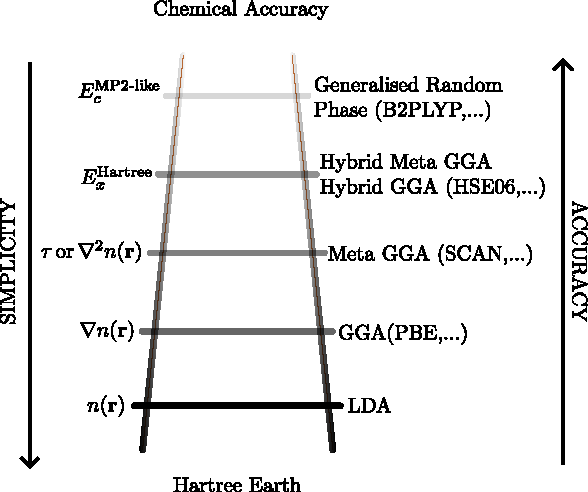
\includegraphics[width=0.6\textwidth]{Jacob-ladder.pdf}
  \caption{Jacob's ladder of exchange-correlation functionals as proposed by J. Perdew\supercite{Perdew2001}. The ladder categorises the functionals into rungs, from the simplest approximation (LDA) at the bottom, progressing to more sophisticated and accurate approximations (Generalised Random Phase) at the uppermost rung.  
  }
  \label{fig:jacob-ladder}
\end{figure}

%\section{Density Functional Tight Binding}
%This is a placeholder 

\section{Ab initio Molecular Dynamics} 
\label{sec:ab-initio-molecular-dynamics}
Molecular dynamics (MD)\supercite{marx2009ab, Kuhne2014} is a widely used computational method that allows us to simulate a many-body condensed matter system and compute its thermodynamic and dynamical properties. In MD, a system is modelled as a collection of particles---atoms or molecules--- whose trajectories evolve under the influence of interatomic forces following Newton's equations of motion. 


One of the most challenging yet crucial aspects of MD is calculating the interatomic forces. In classical MD, these forces are typically computed using predefined potential functions or force fields, either constructed upon empirical data or from independent electronic structure calculations that have been parameterised to reproduce experimental or \emph{ab initio} data for small reference systems. Despite their fair success---which we acknowledge but shall not discuss in detail---these empirical interatomic potentials are often limited in their accuracy and transferability. Certain atoms, molecules, or even large systems may give rise to highly complex interatomic interactions that, if attempted to be modelled with empirical potentials, would require a significant amount of effort. Likewise, these potentials are very often limited to a narrow range of configurations, making them ill-suited for processes involving significant structural changes, such as phase transitions or large deformations.  

Therewith, classical MD can be extended by a first-principles approach, where the interatomic forces are computed on-the-fly from accurate electronic structure calculations, ultimately leading to \emph{ab initio} molecular dynamics (AIMD). This approach enables us to overcome the limitations outlined for classical MD, albeit at a significant computational cost. AIMD employs electronic structure methods, such as DFT, to compute the interatomic forces at each time step, without relying on predefined interatomic potentials, thereby providing AIMD with improved predictive power and flexibility.  

\subsection{Hellmann-Feynman Theorem}
 The Hellmann-Feynman theorem\supercite{Feynman1939, Politzer2018} establishes a relation between the derivative of the total energy $E$ of a system concerning a parameter $\lambda$ and the expectation value of the derivative of the Hamiltonian with respect to that same parameter.
 While the proof of this theorem is relatively straightforward---as shown later in this section---
 it plays a pivotal role in computing interatomic forces in AIMD. 
 
To this end, let us consider the total energy of a system 
\begin{equation}
	\label{69}
	E = \langle \Psi \big| \hat{H} \big| \Psi \rangle
\end{equation}
If $\lambda$ is a parameter that appears explicitly in the Hamiltonian, then 
\begin{equation}
	\label{eq70}
\begin{aligned}
	\frac{\partial E}{\partial \lambda} &= \frac{\partial}{\partial \lambda} \langle \Psi \big| \hat{H} \big| \Psi \rangle \\
  &= \bigg\langle \Psi \bigg| \frac{\partial \hat{H}}{\partial \lambda} \bigg| \Psi \bigg\rangle + \bigg\langle \frac{\partial \Psi}{\partial \lambda} \bigg| \hat{H} \bigg| \Psi \bigg\rangle +  \bigg\langle \Psi \bigg| \hat{H} \bigg|  \frac{\partial \Psi}{\partial \lambda}  \bigg\rangle
\end{aligned}
\end{equation}
Provided that $\hat{H}$ is hermitian and $\Psi$ is an eigenstate of the hamiltonian, $\hat{H}|\Psi\rangle = E|\Psi\rangle$,
Equation \ref{eq70} simplifies to
\begin{equation}
    \label{eq71}
    \begin{aligned}
        \frac{\partial E}{\partial \lambda} &= 
    \bigg\langle \Psi \bigg| \frac{\partial \hat{H}}{\partial \lambda} \bigg| \Psi \bigg\rangle + 
    \bigg\langle \frac{\partial \Psi}{\partial \lambda}\bigg| \hat{H} \bigg| \Psi \bigg\rangle +  
    \bigg\langle\frac{\partial \Psi}{\partial \lambda}\bigg|\hat{H}\bigg|\Psi \bigg\rangle \\
    &=\bigg\langle \Psi \bigg| \frac{\partial \hat{H}}{\partial \lambda}
        \bigg| \Psi \bigg\rangle + E\frac{\partial}{\partial \lambda}
        \langle \Psi|\Psi \rangle + E\frac{\partial}{\partial \lambda}
        \langle \Psi|\Psi \rangle \\
    \end{aligned}
\end{equation}
where the last two terms add up to zero, so that Equation \ref{eq71} becomes,
\begin{equation}
    \label{eq72}
    \frac{\partial E}{\partial \lambda} = 
    \bigg\langle \Psi \bigg| \frac{\partial \hat{H}}{\partial \lambda} \bigg| \Psi \bigg\rangle 
\end{equation}
yielding the Hellmann-Feynman theorem. 

When $\lambda$ corresponds to the position of a nucleus, the negative 
derivative of the total energy with respect to $\lambda$ results 
in the force acting on that nucleus. More 
generally, the force on nucleus $I$ can be expressed as 
the negative gradient of the total energy with respect to its position $R_I$,
\begin{equation}
    \label{eq73}
    \mathbf{F}_I = -\nabla_{R_I} \langle \Psi | \hat{H} | \Psi \rangle
\end{equation}
This result---referred to as the Hellmann-Feynman force---provides a 
fundamental connection between the quantum mechanical energy landscape and the 
classical nuclei motion in AIMD. 
\subsection{Born-Oppenheimer Molecular Dynamics}
As previously discussed, AIMD relies on solving the static electronic structure 
problem at each time step, given a set of fixed nuclear positions at a certain instant in time.
One approach to achieve this is the so-called Born-Oppenheimer molecular dynamics 
(BOMD)\supercite{Kuhne2014}, wherein the potential energy $E[\{\psi_{i}\}; \mathbf{R}]$ 
is minimised at each time step with respect to the single-electron wavefunctions
$\{\psi_{i}(\mathbf{r})\}$ under the orthonormality constraint 
$\langle \psi_i(\mathbf{r}) | \psi_j(\mathbf{r}) \rangle = \delta_{ij}$. 
The result is a potential energy surface on which the nuclei evolve classically.

This leads to the following Lagrangian
\begin{equation}
    \label{eq74}
    \mathcal{L}_{\text{BO}}(\{\psi_{i}\}; \mathbf{R}, \dot{\mathbf{R}}) =
    \frac{1}{2}\sum_{I} M_{I} \dot{\mathbf{R}}_{I}^2 - \min_{\{\psi_{i}\}} E[\{\psi_{i}(\mathbf{r})\}; \mathbf{R}]
    + \sum_{ij} \lambda_{ij} \left( \langle \psi_i | \psi_j \rangle - \delta_{ij} \right)
\end{equation}
where the first term on the right-hand side corresponds to the classical kinetic energy of the nuclei. The second term,
$E[\{\psi_{i}\}; \mathbf{R}] = E^{\text{KS}}[\{\psi_{i}[n(\mathbf{r})]\}; \mathbf{R}] + E_{II}$, is the total potential energy consisting of the Kohn-Sham ground-state energy and the nuclear-nuclear interaction energy.

By applying the Euler-Lagrange equations to Equation \ref{eq74}
\begin{equation}
    \label{eq75}
\begin{aligned}
    \frac{d}{dt}\frac{\partial \mathcal{L}}{\partial \dot{\mathbf{R}}_{I}} =& \frac{\partial \mathcal{L}}{\partial \mathbf{R}_{I}} \\
    \frac{d}{dt}\frac{\partial \mathcal{L}}{\partial \langle\dot{\psi}_{i}|} =& \frac{\partial \mathcal{L}}{\partial \langle\psi_{i}|}
\end{aligned}
\end{equation}
we obtain the equations of motion 
    \begin{align}
        M_{I}\ddot{\mathbf{R}}_{I} &= -\nabla_{\mathbf{R}_{I}} \left[\min_{\{\psi_{i}\}} E[\{\psi_{i}(\mathbf{r})\}; \mathbf{R}]\bigg|_{\{\langle \psi_i(\mathbf{r}) | \psi_j(\mathbf{r}) \rangle = \delta_{ij}\}} \right]\label{eq76} \\
        0 &= -\hat{H}^{\text{KS}}|\psi_{i}\rangle  + \sum_{j} \lambda_{ij} | \psi_j \rangle \label{eq77}
    \end{align}
where Equation \ref{eq76} corresponds to the classical Newtonian equations of motion for the nuclei, and Equation \ref{eq77} represents the Kohn-Sham eigenvalue problem.  

Finally, AIMD simulations may also include temperature control, which can be achieved by coupling a thermostat to the system in order to simulate different thermodynamic ensembles---\emph{e.g.}, canonical (NVT) or isothermal-isobaric (NPT) ensembles.
However, the details of thermostats and different ensembles are beyond the scope of this report, and we shall refer the reader to the literature\supercite{tuckerman2023statistical,frenkel2023understanding} for a more detailed discussion of these topics.

\section{Computational Implementation in VASP}
\label{sec:computational-implementation-in-vasp}
The computational studies presented in this report were performed using the Vienna Ab initio Simulation Package (VASP). This is a software suited for performing \emph{ab initio} quantum mechanical calculations\supercite{https://doi.org/10.1002/jcc.21057}. It employs DFT as the basic method, albeit it also allows for beyond-DFT methods such as hybrid functionals, many-body perturbation theory (the GW method), and random phase approximation (RPA). 

VASP is widely adopted in areas such as materials science, condensed matter physics, and quantum chemistry, owing to its demonstrated accuracy and state-of-the-art methods. Consequently, this section is devoted to explaining some important aspects of VASP, with great emphasis on the computational methods employed in this work. 

\subsection{Pseudopotentials}
A crucial step in defining the wavefunctions that describe an atom is the effective modeling of the electron-ion potential. In this context, core electrons represent a challenge since their rapidly oscillating wavefunctions require a denser real-space grid and a larger number of basis functions to be accurately represented.

To circumvent this problem, we first need to consider the fact that core electrons are tightly bound and do not participate in chemical bonding. Therefore, we can treat them as frozen---\emph{i.e.}, keeping them in their ground state and isolated from the solid-state environment---focusing the calculations on valence electrons, as they do participate in chemical bonding and determine the material's properties. Nonetheless, any adopted approximation must adequately account for the influence of core electrons on the valence states, such as screening and exchange interactions.

To this end, we shall introduce the concept of pseudopotentials\supercite{Hellmann1935}. This approximation aims to describe the valence electrons without explicitly treating the core states, replacing the strong Coulomb potential near the nucleus with a weaker one. We begin by separating the single-electron states into valence and core states, denoted as $|\psi_{v}\rangle$ and $|\psi_{c}\rangle$, respectively. We then define a new set of valence states $|\tilde{\psi}_{v}\rangle$  through the following relation 
\begin{equation}
    \label{eq78}
    |\tilde{\psi}_{v}\rangle = |\psi_{v}\rangle + \sum_{c} |\psi_{c}\rangle 
    \langle \psi_{c} |\tilde{\psi}_{v}\rangle
\end{equation}
Applying the single-particle Hamiltonian $H^{sp}$ to the pseudo-valence states, and taking into account that $|\psi_{v}\rangle$ and $|\psi_{c}\rangle$ are eigenstates of the single-particle Hamiltonian, we get
\begin{equation}
    \label{eq79}
    \begin{aligned}
    H^{sp} |\tilde{\psi}_{v}\rangle &= H^{sp}|\psi_{v}\rangle  + 
    \sum_{c} H^{sp}|\psi_{c}\rangle \langle \psi_{c} |\tilde{\psi}_{v}\rangle\\
    &= \epsilon_{v} |\psi_{v}\rangle + \sum_{c} \epsilon_{c} |\psi_{c}\rangle
    \langle \psi_{c} |\tilde{\psi}_{v}\rangle\\
    &= \epsilon_{v} |\psi_{v}\rangle + \sum_{c} (\epsilon_{c} - \epsilon_{v}) |\psi_{c}\rangle
    \langle \psi_{c} |\tilde{\psi}_{v}\rangle\\
    \end{aligned}
\end{equation}
Rearranging the terms, we obtain the following expression
\begin{equation}
    \label{eq80}
    \left[H^{sp} + \sum_{c} (\epsilon_{v} - \epsilon_{c})|\psi_{c}\rangle \langle \psi_{c} | \right] 
    |\tilde{\psi}_{v}\rangle = \epsilon_{v} |\tilde{\psi}_{v}\rangle
\end{equation}
Equation \ref{eq80} describes the Hamiltonian of the pseudo-valence states, which we can define as 
\begin{equation}
    \label{eq81}
    \hat{H}^{ps} = H^{sp} + \sum_{c} (\epsilon_{v} - \epsilon_{c})|\psi_{c}\rangle \langle \psi_{c} |
\end{equation}
The modified potential for these states is called the pseudopotential, given by 
\begin{equation}
    \label{eq82}
    V^{ps}(\mathbf{r}) = V^{sp} + \sum_{c} (\epsilon_{v} - \epsilon_{c})|\psi_{c}\rangle \langle \psi_{c} |
\end{equation}
We emphasise that the pseudo-valence states associated with Equation \ref{eq80} have the same single-particle energies as the valence states, and they remain orthogonal to the core states. However, they are not strictly normalised, which can introduce minor inaccuracies in practical calculations. 

Various pseudopotentials have been proposed to achieve the desired trade-off between accuracy and computational cost. Those pseudopotentials requiring larger cut-off energies---hard pseudopotentials---are better suited for capturing the strong interactions inherent in core electrons. In contrast, soft pseudopotentials are often preferred because they require fewer basis functions, thereby reducing computational cost, albeit at the expense of accuracy.

\subsection{Projector Augmented-Wave (PAW) Method in VASP}
The projector augmented wave (PAW) method---implemented in VASP and used in this work---aims to address some limitations of pseudopotentials by introducing auxiliary functions called projectors, allowing for core and valence electrons to be better represented and enhancing computational efficiency. 

However, before we introduce the PAW formalism---at least to the extent necessary for this report---we shall first introduce some important concepts that underpin the PAW method.
\subsubsection{Key Concepts}
\begin{itemize}
    \item \textbf{Brillouin Zone and k-points}

    Crystalline solids are described in real space in terms of a primitive unit cell (PUC)\supercite{kaxiras2003atomic}, which is the smallest repeating unit capable of generating the entire solid through periodic boundary conditions. It is characterised by a periodic arrangement of lattice points, referred to as the Bravais lattice. All the lattice points are associated with a set of lattice vectors $\mathbf{R}$ formed by all the possible combinations of integer multiples of the primitive lattice vectors 
    $\mathbf{a}_1$, $\mathbf{a}_2$ and $\mathbf{a}_3$

    \begin{equation}
        \label{eq83}
        \mathbf{R} = n_1\mathbf{a}_1 + n_2\mathbf{a}_2 + n_3\mathbf{a}_3, \quad n_1, n_2, n_3 \in \mathbb{Z}
    \end{equation}
    The primitive unit cell is then defined as the volume enclosed by the primitive lattice vectors 
    \begin{equation}
        \label{eq84}
        V_{PUC} = \mathbf{a}_1 \cdot (\mathbf{a}_2 \times \mathbf{a}_3)
    \end{equation}
Using this definition, it is possible to represent the entire crystal by
modelling solely its unit cell. Additionally, to appropriately describe 
electronic properties, we must transition to reciprocal space, defined by
the reciprocal vectors 
\begin{equation}
    \label{eq85}
    \mathbf{b}_1 = \frac{2\pi}{V_{PUC}} (\mathbf{a}_2 \times \mathbf{a}_3), \quad
    \mathbf{b}_2 = \frac{2\pi}{V_{PUC}} (\mathbf{a}_3 \times \mathbf{a}_1), \quad
    \mathbf{b}_3 = \frac{2\pi}{V_{PUC}} (\mathbf{a}_1 \times \mathbf{a}_2)
\end{equation}
that satisfy the condition $\mathbf{a}_{i}\vdot \mathbf{b}_{j} = 2\pi \delta_{ij}$. Any 
reciprocal lattice vector $\mathbf{G}$ can then be expressed as
\begin{equation}
    \label{eq86}
    \mathbf{G} = m_1\mathbf{b}_1 + m_2\mathbf{b}_2 + m_3\mathbf{b}_3, \quad m_1, m_2, m_3 \in \mathbb{Z}
\end{equation}

The reciprocal space is divided into regions called Brillouin zones (BZs). The first Brillouin zone is defined as the region in reciprocal space closest to the origin ($\Gamma$ point). Moreover, the volume of the first BZ is given by
\begin{equation}
    \label{eq87}
    V_{BZ} = \frac{(2\pi)^3}{V_{PUC}}
\end{equation}
which ensures consistency between the real and reciprocal spaces, and proper normalisation when integrating physical quantities over the BZ.

Finally, because electrons in a crystal are subjected to a periodic potential, single-electron wavefunctions follow Bloch's theorem and can be expressed as 
\begin{equation}
    \label{eq88}
    \psi_{\mathbf{k}} = e^{i\mathbf{k} \cdot \mathbf{r}} u_{\mathbf{k}}(\mathbf{r})
\end{equation}
where $\mathbf{k}$ is the wave vector inside the first BZ, and 
$u_{\mathbf{k}}(\mathbf{r}) = u_{\mathbf{k}}(\mathbf{r}+\mathbf{R})$ is a periodic function of the Bravais lattice.
Many quantities---such as the total energy, electronic density and the total density of states---
can be computed by integrating functions of $\mathbf{k}$ over the 
Brillouin zone, 
\begin{equation}
    \label{eq89}
    \langle A \rangle = \frac{V_{PUC}}{(2\pi)^3} \int_{BZ} A(\mathbf{k}) d\mathbf{k}
\end{equation}
Attempting to compute this integral over the entire BZ would require an infinite number of $\mathbf{k}$ points, which is intractable in practice. Instead, we can discretise the BZ into a finite number of $\mathbf{k}$ points. In VASP, it is achieved by following the Monkhorst-Pack\supercite{Monkhorst1976} scheme, 
\begin{equation}
    \label{eq90}
    \mathbf{k} = \sum_{i=3}^{3} \frac{n_i + s_i + \frac{1 - N_i}{2}}{N_1} \mathbf{b}_i 
\end{equation}
where $n_i$ are indices representing the subdivisions along each reciprocal lattice vector, $s_i$ is an optional shift in terms of subdivisions, and $N_i$ is the total number of subdivisions along the $\mathbf{b}_i$ direction. 
 
Ultimately, the Monkhorst-Pack scheme allows us to generate a uniform and symmetrical grid of $\mathbf{k}$ points in the BZ, and, consequently, to compute integrals over the BZ by summing over a finite number of $\mathbf{k}$ points. 

    \item \textbf{Plane-Wave Expansion and Cut-off Energy}  
    
Following from our previous discussion---where we expressed the single-electron wavefunction as a combination of a periodic function and a plane wave---we can expand $u_{\mathbf{k}}(\mathbf{r})$ in terms of a set of plane waves 
\begin{equation}
\label{eq91}
    u_{\mathbf{k}}(\mathbf{r}) = \sum_{\mathbf{G}} C_{\mathbf{G}} e^{i\mathbf{G} \cdot \mathbf{r}}
\end{equation}

Combining Equations \ref{eq88} and \ref{eq91}, gives 
\begin{equation}
    \label{eq92}
    \psi_{\mathbf{k}}(\mathbf{r}) =
    \sum_{\mathbf{G}} C_{\mathbf{k+G}} e^{i(\mathbf{k} + \mathbf{G}) \cdot \mathbf{r}}
\end{equation}
where $C_{\mathbf{k+G}}$ are the corresponding Fourier coefficients 
associated to the plane wave of wavevector $\mathbf{k} + \mathbf{G}$.

Noticeably, Equation \ref{eq92} introduces a new complexity in the calculations---the evaluation of a single k-point requires the summation over an infinite number of possible $\mathbf{G}$ vectors. However, the interpretation of Equation \ref{eq92} as solutions to the Schrödinger equation allows for the kinetic energy to be expressed as
\begin{equation}
    \label{eq93}
    E_{\text{kin}} = \frac{1}{2} |\mathbf{k} + \mathbf{G}|^2
\end{equation}
In practice, lower energy solutions are more physically relevant, thereby allowing us to truncate the infinite summation by including only plane waves whose kinetic energy does not exceed a certain cut-off energy
$E_{\text{cut}}$
\begin{equation}
\label{eq94} 
\frac{1}{2} |\mathbf{k} + \mathbf{G}|^2 \leq E_{\text{cut}}
\end{equation}
This gives a finite expansion
\begin{equation}
    \label{eq95}
    \psi_{\mathbf{k}}(\mathbf{r}) = \sum_{|\mathbf{k} + \mathbf{G}|^2/2 \leq E_{\text{cut}}}
C_{\mathbf{k}+\mathbf{G}} \, e^{i(\mathbf{k} + \mathbf{G}) \cdot \mathbf{r}}
\end{equation}
Finally, in VASP, we often set the cut-off energy based on a convergence criterion of the total energy of the system 
\begin{equation}
\label{eq96}
    \Delta E_{tot} < 1 \text{meV/atom}
\end{equation}
ensuring a good description of the electronic structure of the system and keeping the calculations computationally feasible.

\end{itemize}

\subsubsection{Projector Augmented-Wave (PAW) Method}
Having explored the base concepts of the Projector Augmented-Wave (PAW) method---regarding its implementation in VASP---we can transition to the PAW formalism itself.  P. E. Bl\"ochl\supercite{Blochl1994} first introduced the PAW method  as a generalisation of the pseudopotential method and linear augmented plane-wave method. Later on, it was further refined by G. Kresse and J. Joubert\supercite{Kresse1999}, providing a formal relationship between ultra-soft pseudopotentials and the PAW method. 

The PAW method addresses the problem of describing the valence states with high accuracy while accounting for the large variations in the all-electron (AE) wavefunction near the atomic core. It does so by introducing a transformation that maps pseudo (PS) wavefunctions---smooth and computationally efficient---onto their corresponding AE counterparts. Thereby, any AE Kohn-Sham wavefunction $\Psi_n$ can be recovered from a PS wavefunction $\tilde{\Psi}_n$ by means of a linear tranformation
\begin{equation}
    \label{eq97}
    \ket{\Psi_n} = |\tilde{\Psi}_n\rangle + \sum_{i} \left( 
        \ket{\phi_i} - |\tilde{\phi}_i\rangle \right)
        \langle \tilde{p}_i | \tilde{\Psi}_n \rangle
\end{equation}
where important elements are to be highlighted:
\begin{itemize}
    \item AE partial wavefunctions $\ket{\phi_i}$, obtained from a reference atom. 
    \item PS partial wavefunctions $|\tilde{\phi}_i\rangle$, which match the AE wavefunctions outside a core radius $r_c$
    \item Projector functions $\ket{\tilde{p}_i}$, which quantify the contribution of the difference $\ket{\phi_i} - |\tilde{\phi}_i\rangle$ to be added to the PS wavefunction in order to recover the AE wavefunction. They fulfil the biorthonormality condition $\langle \tilde{p}_i | \tilde{\phi}_j \rangle = \delta_{ij}$ within the augmented region, ultimately leading to the completeness relation $\sum_i |\tilde{\phi}_i\rangle \langle \tilde{p}_i| = \mathbb{1}$ .
\end{itemize}
Additionally, in the PAW method, the total AE electronic density is expressed as 
\begin{equation}
    \label{eq98}
    n(\mathbf{r}) = \tilde{n}(\mathbf{r}) + n^1(\mathbf{r}) - \tilde{n}^1(\mathbf{r})
\end{equation}
where $\tilde{n}$ is the PS valence electronic density, $n^1$ is the AE one-center electronic density accounting for the contribution of the valence states inside the augmentation region, and $\tilde{n}^1$ is the corresponding PS one-center electronic density.

Finally, the PAW method helps us to recover the true AE electronic density by correcting the PS electronic density within the augmentation region. As a result, many electronic structure properties---such as the total energy, forces, and stresses---can be accurately evaluated.

\subsection{Equation of State (EOS)}
To study the mechanical properties of bulk materials, it is essential to establish a relationship between observables---such as the ground-state total energy---and macroscopic variables like volume or pressure. In this context, the third-order Birch-Murnaghan equation of state\supercite{Birch1947,poirier2000introduction} provides a means to relate the total energy to the change in volume in the system. By fitting energy-volume data to this equation, one can obtain important elastic properties, including equilibrium volume and energy, the bulk modulus, and its pressure derivative. This equation is given by 
\begin{equation}
    \label{eq99}
     E(V) = E_0 + \frac{9}{16} V_0 B_0 \left\{ \left[ \left( \frac{V_0}{V} \right)^{2/3} 
     - 1 \right]^3 B_0' + \left[ \left( \frac{V_0}{V} \right)^{2/3} - 1 \right]^2 \left[6 - 4 \left( \frac{V_0}{V} \right)^{2/3} \right] \right\}
\end{equation}
where $E_0$, $V_0$, $B_0$, and $B_0'$ are the equilibrium energy, volume, bulk modulus, and its pressure derivative, respectively.

Equation \ref{eq99} is utilised in this work to report the aforementioned thermodynamic properties, which are essential for understanding the material's mechanical response under compression or expansion. 

\subsection{Machine Learning Force Fields (MLFFs)}
In an earlier discussion, we introduced the concept of \emph{ab initio} molecular dynamics (AIMD) and highlighted its importance for determining the dynamical properties of a material. Nonetheless---even though VASP is highly optimized for these calculations---AIMD methods remain computationally expensive, restricting their applicability to small simulation cells and short simulation times. 

In this regard, machine learning force fields (MLFFs) represent a promising alternative. These models are trained on accurate \emph{ab initio} datasets, enabling them to learn the underlying potential energy and produce fast and accurate predictions of atomic energies, forces, and stresses. MLFFs can drastically reduce computational cost while minimising any human intervention and expertise required for the force field construction.

In VASP, MLFFs are implemented following an on-the-fly machine learning algorithm\supercite{Jinnouchi2019} (see Figure \ref{fig:MLFF-pipeline}). To construct the machine-learning force field, several structure datasets are required. A structure dataset must define the Bravais lattice, atomic positions, total energy, forces, and the stress tensor computed from first principles (FP). Given the datasets, local configurations around an atom are identified and mapped onto a set of descriptors \supercite{Jinnouchi2020}, describing the local environment around each atom in terms of an atomic distribution function.

\begin{figure}[H]
    \centering
    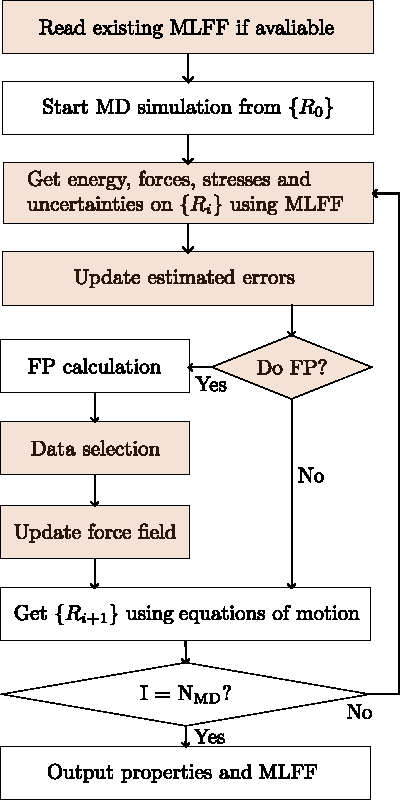
\includegraphics[width=0.4\textwidth]{MLFF-pipeline.pdf}
    \caption{On-the-fly force field generation pipeline in VASP\supercite{Jinnouchi2019}. First, the algorithm reads the existing MLFF if available; otherwise, it generates a new one. If accurate enough, a new structure is generated using the force field; otherwise, a first-principles calculation is performed. If the predicted uncertainty is too large, the new structure is added to the dataset, and the force field is retrained. This oscillating process between training and prediction continues until the total number of ionic steps specified in the setup is reached.}
    \label{fig:MLFF-pipeline}
\end{figure}
\begin{align}
    \rho_{i}^{(2)}(r) &= \frac{1}{4\pi} \int \rho(r\hat{\mathbf{r}}) d\hat{\mathbf{r}} \label{eq100} \\
    \rho_{i}^{(3)}(r, s, \theta) &= \iint d\hat{\mathbf{r}} d\hat{\mathbf{s}} 
    \, \delta (\hat{\mathbf{r}} \vdot \hat{\mathbf{s}}-\cos{\theta})
    \sum_{j\neq 1}^{\text{N}_{a}}\sum_{k\neq i,j}^{\text{N}_{a}}
    \tilde{\rho}_{ij}(r\hat{\mathbf{r}})\tilde{\rho}_{ik}(s\hat{\mathbf{s}}) \label{eq101}
\end{align}
Equation \ref{eq100} defines the two-body descriptor as the probability of finding an atom $j(j\neq i)$ at a distance $r$ from atom $i$. Conversely, Equation \ref{eq101} is known as the three-body descriptor and describes the probability to find an atom $j(j\neq i)$ at a distance $r$ from atom $i$ and another atom $k(k\neq i,j)$ at a distance $s$ from atom $i$ spanning an angle $\angle kij$ between them. These descriptors are then used to construct the local potential energy functionals $U_{i}=F[\rho_{i}^{(2)}, \rho_{i}^{(3)}]$ upon which the force field is constructed. 

The force field is then generated during AIMD simulations following the steps below:
\begin{enumerate}
    \item The machine predicts the energy, forces, stress tensor, and uncertainty for the current atomic configuration using the available force field. 

    \item The algorithm decided whether to perform an FP calculation or not. This decision is based on the uncertainty of the prediction. If the uncertainty exceeds a predefined threshold, the machine proceeds to step 3; otherwise, it continues to step 5. 

    \item The FP calculation is performed for the current structure, and the obtained dataset is then stored as a candidate for the training dataset. 

    \item If the number of candidate structures reaches a certain threshold, or if the uncertainty becomes too large, the algorithm updates the training set and generates a new force field. 

    \item Update the atomic positions and velocities. If the force field is not accurate enough, the FP energy, forces, and stress tensor are used. Otherwise, those predicted by the force field are used. Afterwards, the algorithm returns to step 1 until the total number of ionic steps is reached.
\end{enumerate}

Ultimately, MLFFs provide a robust and efficient method for performing MD simulations. It combines the accuracy of AIMD with the speed of classical MD, allowing for large and complex condensed matter systems to be studied with remarkable accuracy and efficiency.

\section{Density Functional Tight Binding (DFTB+)}
\label{sec:dftb}
Density Functional Tight Binding (DFTB) implemented in the DFTB+ code\supercite{Hourahine2020} is a semi-empirical method derived from the Kohn-Sham DFT by performing a Taylor expansion of the total energy functional around a reference electronic density. This method is computationally efficient, allowing for simulations involving large systems and long timescales with reasonable accuracy, and is significantly faster compared to \emph{ab initio} methods. In this work, the GFN1-xTB (Geometry, Frequency, Noncovalent – extended Tight Binding) method was used to perform an initial relaxation prior to the full structure relaxation using VASP.

\chapter{Methodology}
\label{Chapter3}
\lhead{Chapter 3. \emph{Methodology}}  
This chapter outlines the methodology followed in this work to perform the computational simulations of calcium silicate hydrates ( C--S--H). All the calculations were carried out using Density Functional Tight Binding (DFTB+)---primarily in the initial stages---and subsequently with the Vienna Ab-initio Simulation Package (VASP). All the computational parameters---\texttt{INCAR} files---used for core DFT calculations are detailed in Appendix \ref{AppendixB}.

We begin by describing the initial  C--S--H structure, followed by the 
details of the VASP workflow, emphasising the self-consistent field (SCF) cycle. We then present the main input and output files required for the simulations. Next, we discuss the structure relaxation procedure, which includes an initial relaxation using DFTB+ followed by a full structure relaxation with VASP. Finally, we discuss the generation of the machine learning force field (MLFF), covering the training, refinement, and testing phases. 

\section{Initial  C--S--H Structure}
\label{sec:csh-structure}
The structure used for our investigations of calcium silicate hydrates ( C--S--H) is the molecular model proposed by Pellenq \emph{et al.} \cite{Pellenq2009}. This model was constructed with the chemical composition as the overriding constraint. As such, the model has a calcium/silicon ratio (C/S) of 1.7, and a density of 2.6 g/cm$^3$; consistent with experimental observations. 

It was derived from a monoclinic periodic cell of dry tobermorite, from which SiO$_2$ groups were removed to achieve an experimental C/S ratio. Thereafter, the structure was relaxed using a core-shell potential model at 0 K. Finally, a Grand Canonical Monte Carlo simulation of water adsorption was carried out at 300 K, reporting a chemical composition of (CaO)$_{1.65}$(SiO$_2$)(H$_2$O)$_{1.75}$. 

The model, shown in Figure \ref{fig:csh_structure}, contains
99 calcium (Ca), 60 silicon (Si), 323 oxygen (O), and 208 hydrogen (H) atoms, making a total of 690 atoms. It is noteworthy that the model is not regarded as a perfect representation of  C--S--H, but rather as a good approximation that captures the essential features of cement hydrates.

\begin{figure}[h]
    \centering
    \includegraphics[width=1\textwidth]{POSCAR-extra-colours.png}
    \caption{Molecular model of  C--S--H proposed by Ref. \cite{Pellenq2009}. Lavender and white spheres are oxygen and hydrogen from water molecules, respectively; light blue and brown spheres are inter- and intra-layer calcium ions, respectively; electric blue and red spheres are silicon and oxygen atoms from silica tetrahedra, respectively.}
    \label{fig:csh_structure}
\end{figure}

\section{VASP Workflow}
\label{sec:vasp-workflow}
Most of our calculations were performed using the Vienna Ab Initio Simulation Package (VASP). A central part of the VASP workflow is the self-consistent field (SCF) cycle, illustrated in Figure~\ref{fig:vasp_workflow}. This cycle is essential for structure relaxation, \emph{ab initio} molecular dynamics (AIMD) simulations, and other DFT calculations. We hereby present the main procedure of the SCF cycle:

\begin{itemize}
    \item At the beginning of the cycle, a trial electronic density is generated---either from a previous calculation or from an initial guess. 
    \item The algorithm then proceeds to construct the effective potential, defined as the sum of the Hartree, external, and exchange-correlation potentials. The latter is specified by the user (e.g., PBEsol, HSE06).
    \item VASP then solves the Kohn-Sham equation, generating a new set of single-electron wavefunctions at each iteration. 
    \item A new electronic density is calculated from the wavefunctions. This process repeats until self-consistency is achieved---\emph{i.e.}, the total energy difference between consecutive iterations falls below a predefined tolerance. The user sets this value, and for our calculations, values of \texttt{EDIFF=1E-5} and \texttt{EDIFFG=-0.02} were used. 
\end{itemize}

\begin{figure}[h]
    \centering
    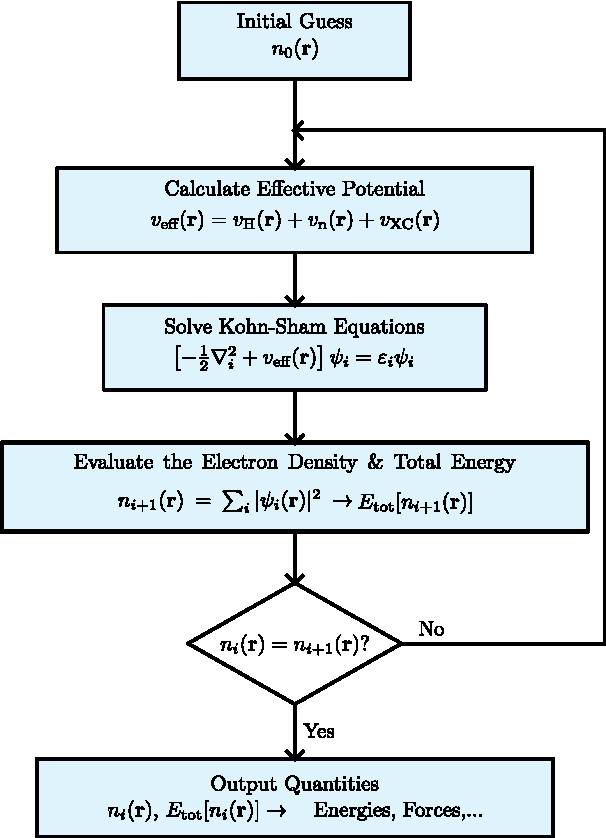
\includegraphics[width=0.6\textwidth]{vasp-workflow.pdf}
    \caption{
        Self-consistent field (SFC) cycle in VASP for DFT calculations adapted from Ref. \cite{sholl2023density}. The entire cycle starts with an initial guess of the electronic density $n_0(\mathbf{r})$, which is then used to calculate the effective potential $v_{\text{eff}}(\mathbf{r})$. Then, the resulting potential is used to solve the Kohn-Sham equations, from which single-electron wavefunctions $\psi_i(\mathbf{r})$ are obtained. Consequently, the new electronic density $n_{i+1}(\mathbf{r})$ is calculated. Should the old and new densities be close enough---up to a predefined threshold---the cycle stops, and the final electronic density is used to calculate the energies, forces, and stress tensor of the system. Otherwise, the cycle repeats itself until convergence is achieved. 
    }
    \label{fig:vasp_workflow}
\end{figure}

\section{VASP Input \& Output Files}
\label{sec:vasp-input-output-files}
The VASP input and output files are essential for our calculations. On the one hand, the input files contain necessary information---such as the initial structure, exchange-correlation functionals, PAW pseudopotentials, k-point grid, and convergence criteria---that guide the different simulations. On the other hand, the output files contain the results of the different simulations, such as the total energy, forces, stress tensor, and the fully relaxed structure.

This section provides an overview of the required input files for VASP calculations, as well as some relevant output files. For a detailed and rather technical description of the files described herein, we refer the reader to the VASP manual \cite{zotero-item-672}.

\subsection{Input Files}
\subsubsection{INCAR}
The \texttt{INCAR} file (see Figure \ref{fig:incar}) defines the computational parameters in VASP and specifies the type of calculation to be performed. Each simulation stage---such as structure optimisation, Density of States (DOS) calculations, AIMD simulations, or MLFF training---is defined by a specific set of INCAR tags. 
\begin{figure}[H]  
	\centering  
	\begin{threeparttable}  
		\caption{Example of an \texttt{INCAR} file used for structure relaxation of  C--S--H. This file specifies the optimisation algorithm, force convergence criteria, exchange-correlation functional (PBEsol) and ionic relaxation parameters. Depending on the type of calculation to be performed, different tags may be added or removed.
        }  
		\label{fig:incar}  
		\resizebox{\textwidth}{!}{  
			\begin{tabular}{>{\columncolor{blue!10}}l>{\columncolor{blue!10}}l>{\columncolor{blue!10}}l>{\columncolor{blue!10}}l>{\columncolor{blue!10}}l>{\columncolor{blue!10}}l>{\columncolor{blue!10}}l>{\columncolor{blue!10}}l>{\columncolor{blue!10}}l>{\columncolor{blue!10}}l>{\columncolor{blue!10}}l>{\columncolor{blue!10}}l>{\columncolor{blue!10}}l>{\columncolor{blue!10}}l>{\columncolor{blue!10}}l>{\columncolor{blue!10}}l>{\columncolor{blue!10}}l>{\columncolor{blue!10}}l>{\columncolor{blue!10}}l}  
				\hline   
				\multicolumn{3}{c}{\cellcolor{blue!10} \textbf{GENERAL}} & & & & & & & & & & & & & & & & \\   
				\textbf{SYSTEM} & \textbf{=  C--S--H} & \textit{\# System name} & & & & & & & & & & & & & & & & \\   
				\textbf{PREC}   & \textbf{= Accurate} & \textit{\# Precision level} & & & & & & & & & & & & & & & & \\   
				\multicolumn{3}{c}{\cellcolor{blue!10} \textbf{ELECTRONIC OPTIMIZATION}} & & & & & & & & & & & & & & & & \\   
				\textbf{ENCUT}  & \textbf{= 800} & \textit{\# Plane-wave cutoff (eV)} & & & & & & & & & & & & & & & & \\   
				\textbf{LREAL}  & \textbf{= Auto} & \textit{\# Real-space projection} & & & & & & & & & & & & & & & & \\   
				\textbf{ISMEAR} & \textbf{= 0} & \textit{\# Smearing method} & & & & & & & & & & & & & & & & \\   
				\textbf{SIGMA}  & \textbf{= 0.05} & \textit{\# Smearing width (eV)} & & & & & & & & & & & & & & & & \\   
				\textbf{ALGO}   & \textbf{= F} & \textit{\# Electronic minimization algorithm} & & & & & & & & & & & & & & & & \\   
				\textbf{AMIX}   & \textbf{= 0.1} & \textit{\# Charge density mixing parameter (damping)} & & & & & & & & & & & & & & & & \\   
				\multicolumn{3}{c}{\cellcolor{blue!10} \textbf{EXCHANGE-CORRELATION / FUNCTIONAL}} & & & & & & & & & & & & & & & & \\   
				\textbf{GGA}    & \textbf{= PS} & \textit{\# PBEsol functional} & & & & & & & & & & & & & & & & \\   
				\textbf{IVDW}   & \textbf{= 11} & \textit{\# DFT-D3(zero) vdW correction} & & & & & & & & & & & & & & & & \\   
				\textbf{LASPH}  & \textbf{= .TRUE.} & \textit{\# Non-spherical contributions} & & & & & & & & & & & & & & & & \\   
				\textbf{LMAXMIX}& \textbf{= 4} & \textit{\# Maximum l for charge mixing} & & & & & & & & & & & & & & & & \\   
				\multicolumn{3}{c}{\cellcolor{blue!10} \textbf{CHARGE \& WAVEFUNCTION}} & & & & & & & & & & & & & & & & \\   
				\textbf{LCHARG} & \textbf{= F} & \textit{\# Do not write CHGCAR} & & & & & & & & & & & & & & & & \\   
				\multicolumn{3}{c}{\cellcolor{blue!10} \textbf{IONIC RELAXATION}} & & & & & & & & & & & & & & & & \\   
				\textbf{NELMIN} & \textbf{= 4} & \textit{\# Minimum SCF steps} & & & & & & & & & & & & & & & & \\   
				\textbf{MAXMIX} & \textbf{= 40} & \textit{\# Maximum mixing steps} & & & & & & & & & & & & & & & & \\   
				\textbf{IBRION} & \textbf{= 2} & \textit{\# Ionic relaxation algorithm} & & & & & & & & & & & & & & & & \\   
				\textbf{ISIF}   & \textbf{= 3} & \textit{\# Relax ions + cell shape + volume} & & & & & & & & & & & & & & & & \\   
				\textbf{NSW}    & \textbf{= 700} & \textit{\# Maximum ionic steps} & & & & & & & & & & & & & & & & \\   
				\textbf{EDIFFG} & \textbf{= -0.02} & \textit{\# Convergence criterion (eV/\AA)} & & & & & & & & & & & & & & & & \\   
				\textbf{ADDGRID}& \textbf{= T} & \textit{\# Additional grid for accuracy} & & & & & & & & & & & & & & & & \\   
				\hline  
			\end{tabular}  
		}  
	\end{threeparttable}  
\end{figure}
These parameters control convergence thresholds, exchange-correlation functionals, long-range corrections, ensemble choices, and other simulation parameters. If not specified by the user, VASP uses default values. Nonetheless, for reliable and reproducible results, the main parameters must be tailored to the system and the type of calculation.


\subsubsection{POSCAR}
The \texttt{POSCAR} (see Figure \ref{fig:csh_poscar}) file provides the actual structure to be studied. It is subdivided into several sections, each one providing specific information about the system.
\begin{figure}[H]
\resizebox{\textwidth}{!}{
\begin{tabular}{>{\columncolor{blue!10}}c>{\columncolor{blue!10}}c>{\columncolor{blue!10}}c
>{\columncolor{blue!10}}l>{\columncolor{blue!10}}l>{\columncolor{blue!10}}l>{\columncolor{blue!10}}l
>{\columncolor{blue!10}}l>{\columncolor{blue!10}}l>{\columncolor{blue!10}}l>{\columncolor{blue!10}}l
>{\columncolor{blue!10}}l>{\columncolor{blue!10}}l>{\columncolor{blue!10}}l>{\columncolor{blue!10}}l
>{\columncolor{blue!10}}l>{\columncolor{blue!10}}l>{\columncolor{blue!10}}l>{\columncolor{blue!10}}l
>{\columncolor{blue!10}}l>{\columncolor{blue!10}}l>{\columncolor{blue!10}}l>{\columncolor{blue!10}}l
>{\columncolor{blue!10}}l>{\columncolor{blue!10}}l}
\hline
\multicolumn{3}{l}{\cellcolor{blue!10} \textbf{Ca Si O H}} & & & & & & & & & & & & & & & & & & & & & & \\
\multicolumn{3}{l}{\cellcolor{blue!10}1.0} & & & & & & & & & & & & & & & & & & & & & & \\
13.18335946 & 0.18445997 & 0.00755401 & & & & & & & & & & & & & & & & & & & & & & \\
-16.45244030 & 24.21622147 & -0.00875423 & & & & & & & & & & & & & & & & & & & & & & \\
1.20664987 & -0.82375620 & 23.18729854 & & & & & & & & & & & & & & & & & & & & & & \\
\multicolumn{3}{l}{\cellcolor{blue!10} \textbf{Ca Si O H}} & & & & & & & & & & & & & & & & & & & & & & \\
\multicolumn{3}{l}{\cellcolor{blue!10}99 60 323 208} & & & & & & & & & & & & & & & & & & & & & & \\
\multicolumn{3}{l}{\cellcolor{blue!10}Direct} & & & & & & & & & & & & & & & & & & & & & & \\
0.38821570 & 0.10613519 & 0.29312228 & & & & & & & & & & & & & & & & & & & & & & \\
0.37259751 & 0.56538816 & 0.26881558 & & & & & & & & & & & & & & & & & & & & & & \\
0.37469040 & 0.31600944 & 0.23882914 & & & & & & & & & & & & & & & & & & & & & & \\
0.35542617 & 0.78384113 & 0.38748504 & & & & & & & & & & & & & & & & & & & & & & \\
0.91347068 & 0.11233954 & 0.31634176 & & & & & & & & & & & & & & & & & & & & & & \\
0.90355777 & 0.57838562 & 0.23567872 & & & & & & & & & & & & & & & & & & & & & & \\
0.87836092 & 0.32109531 & 0.25338100 & & & & & & & & & & & & & & & & & & & & & & \\
0.84529168 & 0.81264469 & 0.29236748 & & & & & & & & & & & & & & & & & & & & & & \\
0.11769176 & 0.02588977 & 0.65372010 & & & & & & & & & & & & & & & & & & & & & & \\
\hline
\end{tabular}
}
\caption{Unit cell structure in fractional coordinates for the C--S--H (Calcium Silicate Hydrates) system. The lattice vectors, atomic species (99 Ca, 60 Si, 323 O, 208 H), and the first 9 atomic positions are shown. All coordinates are expressed in direct (fractional) form.}
\label{fig:csh_poscar}
\end{figure}
The first line contains a comment specifying the name of the system or a brief description of it. Lines 2-4 provide the scaling factor and the corresponding lattice vectors. The actual lattice vectors are obtained by multiplying the scaling factor (line 2) by the numbers in lines 3-5. Lines 6-7 specify the atomic species as well as the number of ions of each species. Finally, lines 9-onwards provide the ionic positions in angstroms. 

\subsubsection{KPOINTS}
Defining the k-point grid is an essential and one of the first steps when performing DFT calculations, as the accuracy and convergence of the results depend on it. Figure \ref{kpoints} illustrates the \texttt{KPOINTS} file used in this work. The specified mesh is a $1\times 1\times 1$ Gamma-centered grid, obtained after a convergence test. 
\begin{figure}[H]
\resizebox{\textwidth}{!}{
	\begin{tabular}{>{\columncolor{blue!10}}c>{\columncolor{blue!10}}l>{\columncolor{blue!10}}l>{\columncolor{blue!10}}l>{\columncolor{blue!10}}l>{\columncolor{blue!10}}l>{\columncolor{blue!10}}l>{\columncolor{blue!10}}l>{\columncolor{blue!10}}l>{\columncolor{blue!10}}l>{\columncolor{blue!10}}l>{\columncolor{blue!10}}l>{\columncolor{blue!10}}l>{\columncolor{blue!10}}l>{\columncolor{blue!10}}l>{\columncolor{blue!10}}l>{\columncolor{blue!10}}l>{\columncolor{blue!10}}l>{\columncolor{blue!10}}l>{\columncolor{blue!10}}l>{\columncolor{blue!10}}l>{\columncolor{blue!10}}l>{\columncolor{blue!10}}l>{\columncolor{blue!10}}l>{\columncolor{blue!10}}l>{\columncolor{blue!10}}l>{\columncolor{blue!10}}l>{\columncolor{blue!10}}l>{\columncolor{blue!10}}l>{\columncolor{blue!10}}l>{\columncolor{blue!10}}l>{\columncolor{blue!10}}l>{\columncolor{blue!10}}l>{\columncolor{blue!10}}l>{\columncolor{blue!10}}l>{\columncolor{blue!10}}l>{\columncolor{blue!10}}l} \hline
		\multicolumn{1}{l}{\cellcolor{blue!10} \textbf{ C--S--H kpoints}} & & & & & & & & & & & & & & & & & & & & & & & & & & & & & & & & & & & &\\ 
		\multicolumn{1}{l}{\cellcolor{blue!10}0}& & & & & & & & & & & & & & & & & & & & & & & & & & & & & & & & & & & &\\
		\multicolumn{1}{l}{\cellcolor{blue!10} \textbf{Gamma}}& & & & & & & & & & & & & & & & & & & & & & & & & & & & & & & & & & & &\\ 
		1 1 1& & & & & & & & & & & & & & & & & & & & & & & & & & & & & & & & & & & & \\
		0 0 0& & & & & & & & & & & & & & & & & & & & & & & & & & & & & & & & & & & & \\  \hline
	\end{tabular}
 }
	\centering
	\caption{ C--S--H k-point grid centered at the Gamma point. The values "1 1 1" define the grid dimensions in the $x$, $y$, and $z$ directions. For large systems, a Gamma-centered grid is enough to achieve convergence.}
	\label{kpoints}
\end{figure}

\subsubsection{POTCAR}
The \texttt{POTCAR} file contains the PAW pseudopotentials for each atomic species in the system. As such, it defines how valence electrons interact with the atomic cores. It is constructed by concatenating the individual POTCAR files for each species into a single file. In our work,  we employed the following PAW pseudopotentials from the PAW\_PBE library:
\begin{itemize}
    \item Ca: Ca\_pv ([Ar] 4s$^2$)
    \item Si: Si ([Ne] 3s$^2$ 3p$^2$)
    \item O: O ([He] 2s$^2$ 2p$^4$)
    \item H: H (1s$^1$)
\end{itemize}

\subsection{Output Files}
These are the primary output files generated upon finishing an FP calculation in VASP. They provide core information regarding the performance of the calculations, documenting the simulation and providing the basis for further analysis.
\subsubsection{OUTCAR}
The \texttt{OUTCAR} file is a comprehensive output file that contains detailed information about the VASP calculation. It includes a summary of the input parameters, the evolution of the SCF cycle, the total energy, forces on the atoms, and the stress tensor.
\subsubsection{CONTCAR}
The \texttt{CONTCAR} file records the final atomic positions and lattice vectors after a structure relaxation or optimisation. Additionally, this file may also contain atomic velocities and predictor-corrector information if it was written during an AIMD simulation. It has a compatible format with the \texttt{POSCAR} file, making it possible to use it as an input structure for subsequent calculations.

\subsubsection{DOSCAR}
The \texttt{DOSCAR} file stores the Density of States (DOS) and integrated DOS, expressed in states/eV and cumulative number of states, respectively. This data is beneficial for analysing the electronic properties of the system, and understanding features such as the band gap and the distribution of states across the valence and conduction bands. 
\subsubsection{OSZICAR}
The \texttt{OSZICAR} file records a summary of the electronic and ionic iterations during a DFT calculation. It allows the user to monitor the progress of the SCF cycle convergence, visualise changes in the total energy, and follow the evolution of the ionic relaxation process. 
\subsubsection{ML\_ABN}
The \texttt{ML\_ABN} file contains the training dataset collected during an on-the-fly MLFF training process. As previously described, the MLFF is trained together with an AIMD simulation, where atomic configurations are sampled. Representative configurations are then written to this file, which can be reused to continue the training by renaming it to a \texttt{ML\_AB} file.

\subsubsection{ML\_FFN}
The \texttt{ML\_FFN} file is a binary file that stores the trained machine learning force field (MLFF) model at the end of the training phase. It contains the model parameters, such as weights and hyperparameters, that define the MLFF. The model can be used for prediction or further refinement by renaming it to an \texttt{ML\_FF} file.


\section{Strucure Relaxation}
\label{sec:structure-relaxation}
Relaxing the  C--S--H structure is a crucial step towards obtaining equilibrium properties of this material. This process involves minimising both the forces on atoms and the total energy of the system, leading to a stable configuration. In this work, we performed structure relaxation in two stages: an initial relaxation was conducted using DFTB+, which provided a good starting point for VASP and reduced the computational cost of the full structure relaxation. The second stage consists of a full structure relaxation using VASP. Here we outline both stages of the structure relaxation process.

\subsection{Initial Relaxation with DFTB+}
Given the large size of the  C--S--H structure, it was necessary to perform a preliminary relaxation using the GFN1-xTB method implemented in DFTB+. For this step, we first conducted a k-point convergence test. We then plugged this value into the relaxation script in order to run the structure relaxation. This trick allows us to take our structure closer to its equilibrium configuration, without spending too much time and computational power to do so. This approach is valid because we are not using the final structure as our actual optimised structure, but rather as a means to reduce the computation time required for full structure relaxation in VASP.  

\subsection{Full Structure Relaxation with VASP}
After the rough approximation provided by DFTB+, a full structure relaxation is performed using VASP. To achieve this, we first perform a cut-off energy convergence test, followed by a k-point convergence test. Thereafter, we define the k-point mesh in the \texttt{KPOINTS} file, and the cut-off energy in the \texttt{INCAR} file, where we also specified the PBEsol functional and a force convergence criteria of 0.02 eV/\AA. Once the structure has been fully relaxed, it is used to study the Density of States (DOS) and to train the machine learning force field.

\section{Machine Learning Force Field Generation}
\label{sec:mlff-generation}
This stage is subdivided into three main phases: training, refinement, and testing. In this section, we describe each one of them in detail.
\subsection{Training}
As previously discussed, the MLFF is generated on-the-fly during an AIMD simulation. To begin, we use the \texttt{CONTCAR} file, which contains our relaxed structure, as the input \texttt{POSCAR} file for this step. In the \texttt{INCAR} file some parameters need to be set: \texttt{IBRION=0}, indicates VASP to switch to an AIMD simulation; \texttt{NSW=50000} indicates the number of ionic steps; \texttt{POTIM=2.0} is the MD time step in fs; \texttt{MDALGO=3} tells VASP to use the Langevin thermostat; \texttt{TEBEG=400} sets the temperature (in K) at which the simulation is performed, and \texttt{ISIF=3} allows for positions, cell shape and volume to be~updated. 

Finally, \texttt{ML\_LMLFF=T} and \texttt{ML\_ISTART=0} tags govern the MLFF training process. The former enables the use of machine learning force fields, and the latter tells VASP to generate a new MLFF from scratch. Although the parameters described herein are the most important, additional tags may need to be set depending on the performance of the training phase.

\subsection{Refinement}
The refinement phase allows for improvements to be made in the generated MLFF by tuning the hyperparameters in the model. To this end, we first generate a set of 50000 structures using the force field, from which we uniformly sample 50 configurations. Then we compute the total energy, forces and stress tensor for each one of them in two separate runs. The first run utilises first principles, whereas the second run is performed using the MLFF model. The corresponding data is then postprocessed and the errors between DFT and MLFF results are evaluated using configuration-wise Root Mean Square Error (RMSE) defined as follows:
\begin{subequations}
    \label{eq:rmse_per_conf}
    \begin{align}
        \label{eq:energy_error}
        E^i_{\text{error}} &= \frac{E_i^{\text{DFT}} - E_i^{\text{MLFF}}}{\text{N}_{a}} \\
        \label{eq:force_error}
        F^i_{\text{RMSE}} &= \sqrt{\frac{1}{3\text{N}_{a}}\sum_{j=1}^{\text{N}_{a}}\sum_{k=1}^{3} \left(\mathbf{F}_{ijk}^{\text{DFT}} - \mathbf{F}_{ijk}^{\text{MLFF}}\right)^2} \\
        \label{eq:stress_error}
        S^i_{\text{RMSE}} &= \sqrt{\frac{1}{6} \sum_{\alpha=1}^{3}\sum_{\beta=1}^{3} \left(\sigma_{i\alpha\beta}^{\text{DFT}} - \sigma_{i\alpha\beta}^{\text{MLFF}}\right)^2}
    \end{align}
\end{subequations}
where $i$ indicates the configuration index, $\text{N}_a$ is the number of atoms in the system, $j$ is the atom index, $k$ corresponds to the Cartesian components of the forces, and $\alpha$, $\beta$ are the Cartesian indices of the stress tensor. Note that the energy error does not correspond to a RMSE, but rather to a per-atom energy error. Likewise, global RMSE values for the entire set of configurations are computed as follows:
\begin{subequations}
    \label{eq:rmse_global}
    \begin{align}
        \label{eq:rmse_e}
        E_{\text{RMSE}} &= \sqrt{\frac{1}{\text{N}_s}\sum_{i=1}^{\text{N}_s} \left(E_i^{\text{DFT}} - E_i^{\text{MLFF}}\right)^2} \\
        \label{eq:rmse_f}
        F_{\text{RMSE}} &= \sqrt{\frac{1}{\text{N}_{s}} \sum_{i=1}^{\text{N}_{s}} \left(F^i_{\text{RMSE}} \right)^2} \\
        \label{eq:rmse_s}
        S_{\text{RMSE}} &= \sqrt{\frac{1}{\text{N}_s} \sum_{i=1}^{N_s} \left(S^i_{\text{RMSE}} \right)^2}
    \end{align}
\end{subequations}
where $\text{N}_s$ is the total number of sampled configurations. These results are significant as they provide the means to evaluate the performance of our force field.

Afterwards, we conduct a hyperparameter optimisation in order to improve the performance of the force field. It is noteworthy that VASP provides various hyperparameters that we can optimise; nevertheless, in this work, only two hyperparameters were considered---the two and three-body descriptors---as they directly affect the accuracy of the force field. In this regard, we set \texttt{ML\_MODE=refit} and \texttt{ML\_RCUT1=\#} in the \texttt{INCAR} file. The latter parameter corresponds to the radial descriptor (given in \AA), and is to be modified accordingly to a reasonable range. Thereafter, we use the resulting MLFF file to evaluate the performance of the refitted force field for the given \texttt{RCUT1}. We achieve this by setting \texttt{IBRION=-1} and \texttt{ML\_MODE=run} in the \texttt{INCAR} file. This calculation will return the RMSE for energies, forces, and the stress tensor as a function of the descriptor. The same process is then applied to the angular descriptor \texttt{RCUT2}, and the optimal hyperparameters are chosen to minimise the errors. 

\subsection{Testing}
Following the refinement process, we can utilise the MLFF model to conduct various simulations, including AIMD simulations, structure relaxation, and other DFT calculations. In this work, we used the generated force field to compute the equation of state (EOS) of  C--S--H. Additionally, we also performed a simulated annealing process to obtain a more stable structure and computed its corresponding EOS as well. Finally, various MD simulations were conducted at temperatures of 200, 250, 300, 350, and 400 K to study the transferability of the force field as well as the expansion coefficient of  C--S--H.

\chapter{Results \& Discussion}
\label{Chapter4}
\lhead{Chapter 4. \emph{Results \& Discussion}}

\section{My results}
Hello
\begin{figure}[H]
    \centering
    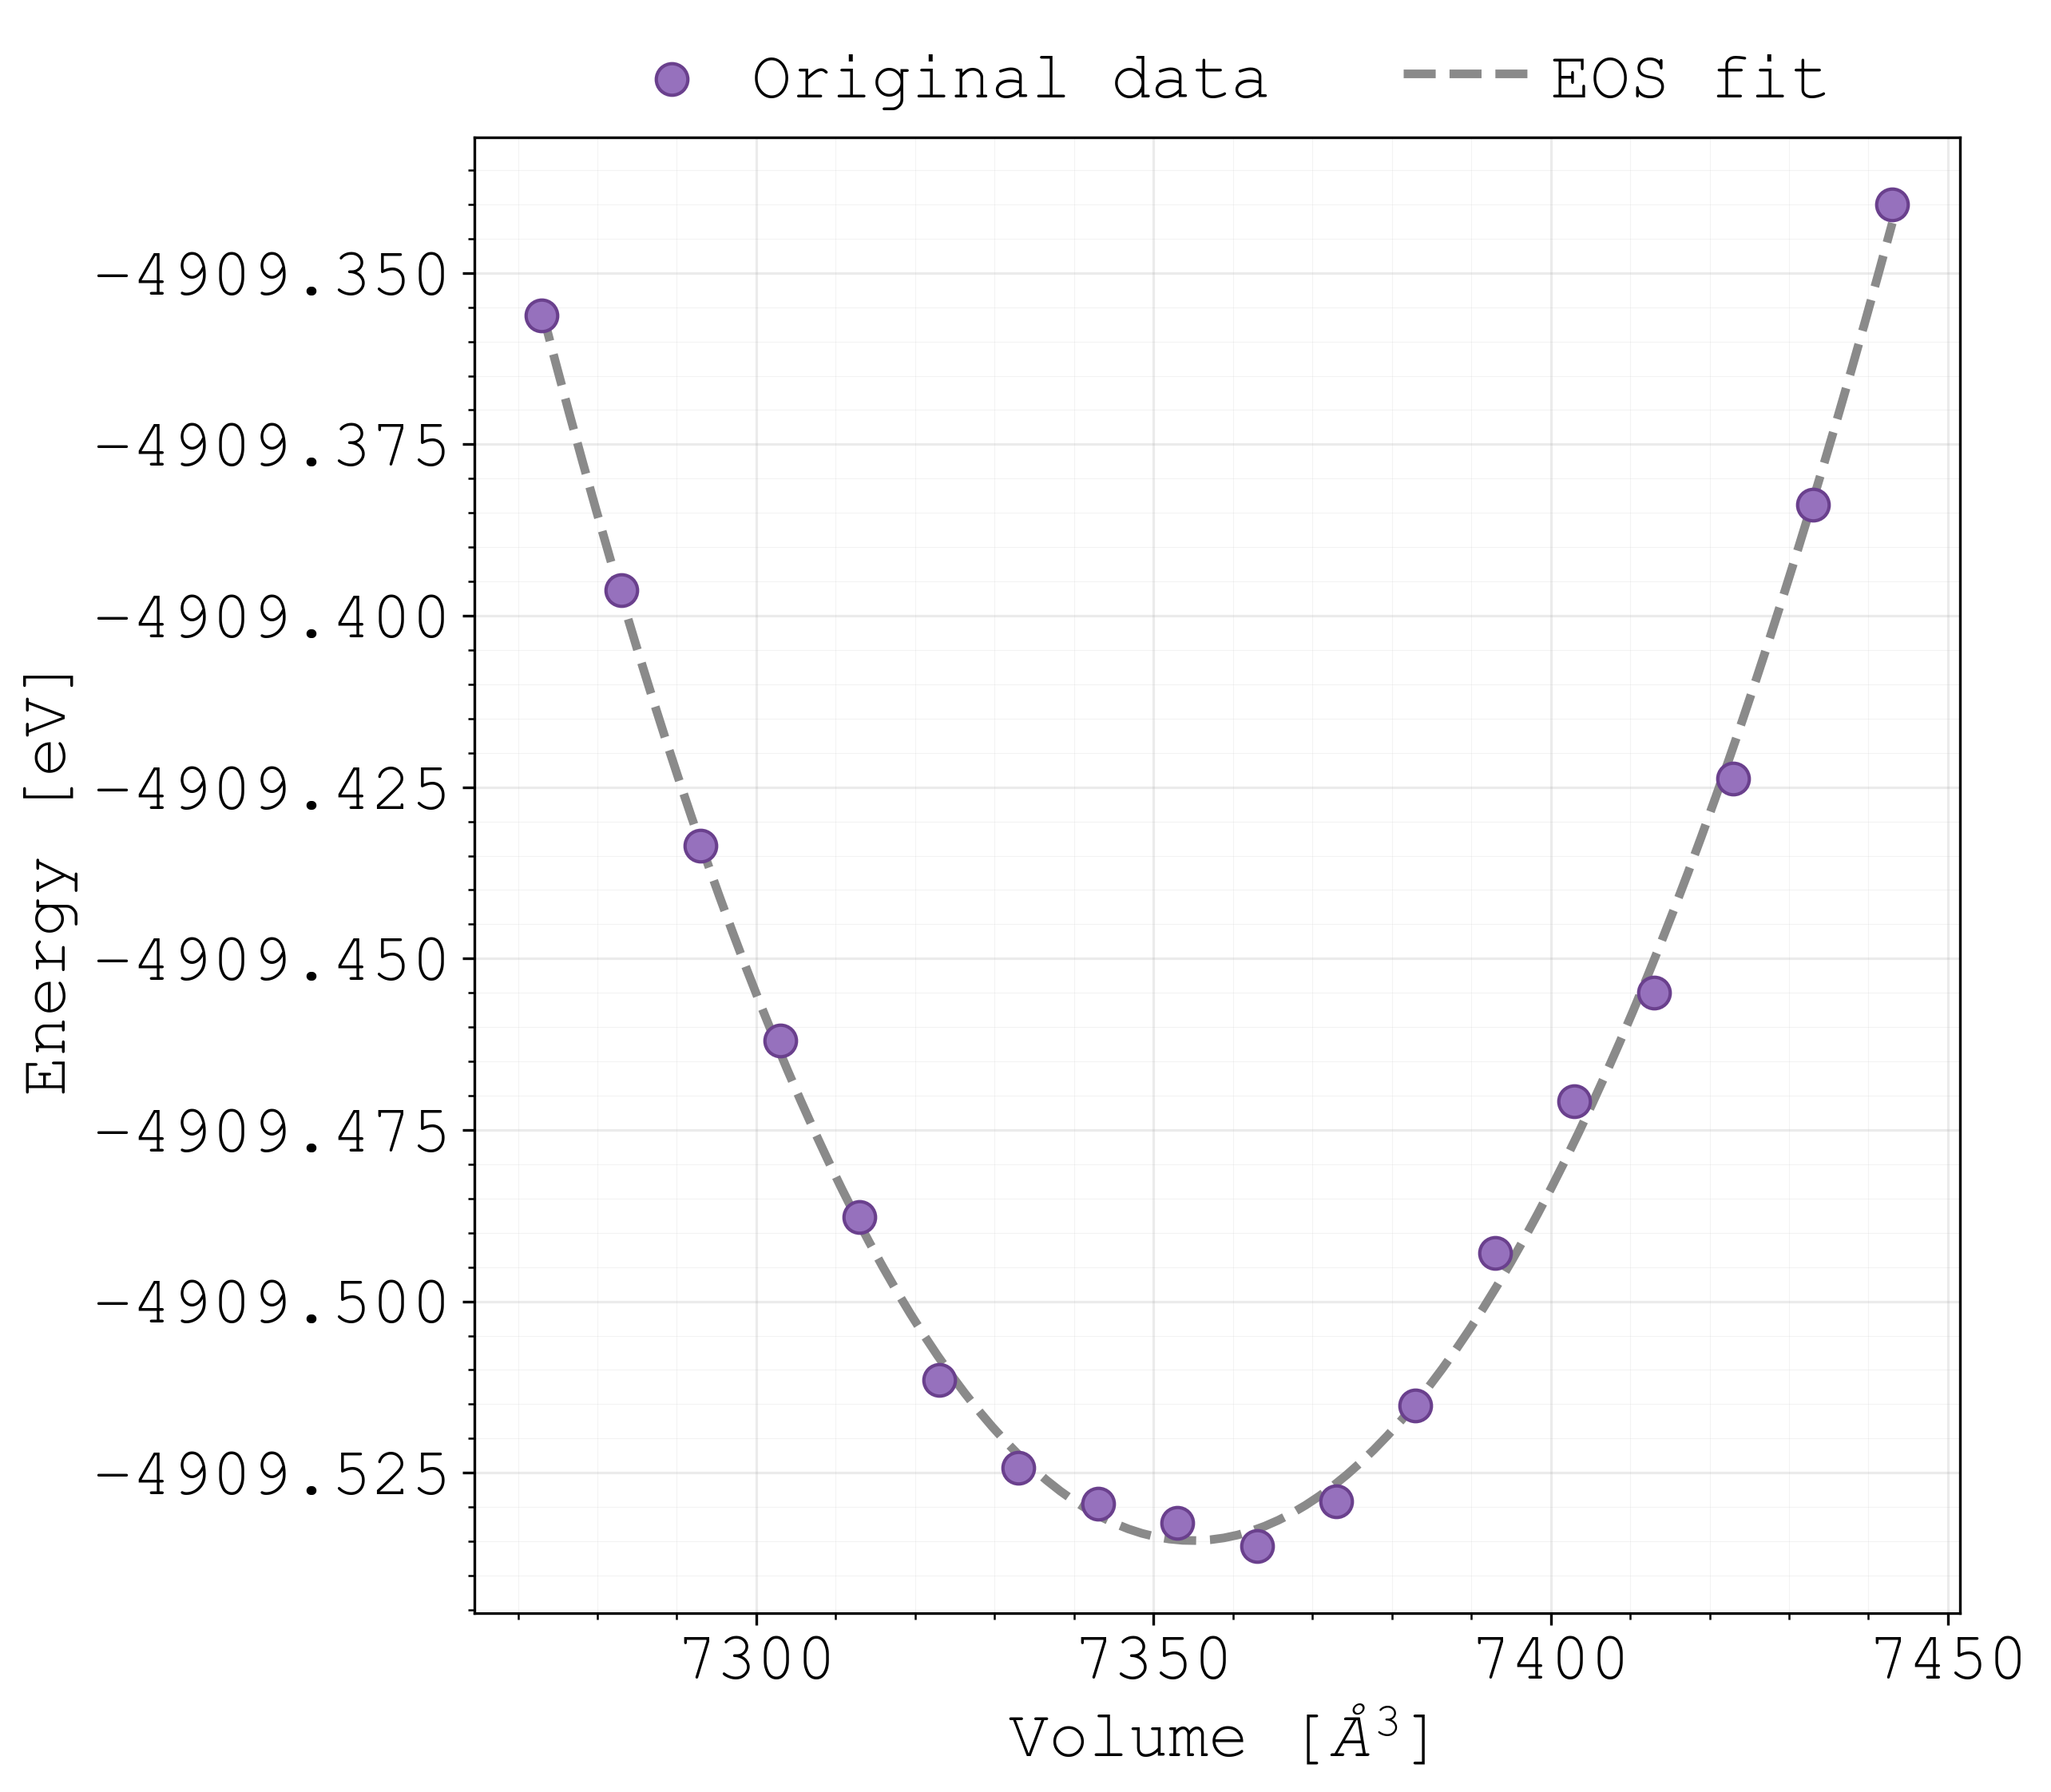
\includegraphics[width=0.5\textwidth]{EOS_SA_EDIFF_02.png}
    \caption{A schematic representation of the DFT formalism. The many-body wavefunction is replaced by a single-particle wavefunction, which is used to calculate the electron density. The electron density is then used to calculate the total energy of the system. Adapted from \supercite{giustino2014materials}.}
    \label{fig:dft}
\end{figure}

\chapter{\texorpdfstring{Conclusions $\&$ Outlook}{Conclusions \& Outlook}} % Main chapter title

\label{Chapter5} % For referencing the chapter elsewhere, use \ref{Chapter5}
\lhead{Chapter 5. \emph{Conclusions $\&$ Outlook}} % This 

In this work, we successfully integrate first-principles calculations with machine learning techniques to develop a robust and efficient machine learning force field (MLFF) tailored for calcium silicate hydrates (C-S-H). The MLFF was constructed using an on-the-fly training approach within \emph{ab initio} molecular dynamics (AIMD) simulations, enabling the accurate modeling of the atomic and mechanical properties of C-S-H. Starting with geometric relaxation of the C-S-H structure using VASP and the PBEsol exchange-correlation functional, we employed a systematic workflow to train, evaluate, and refine the MLFF. This refined force field was then used to compute key thermodynamic properties, including the equation of state (EOS) and mechanical parameters such as the bulk modulus.

Comparisons across different MLFF variants and with available experimental data demonstrated the critical importance of the refinement step in enhancing model accuracy and transferability.
Our final MLFF showed good agreement with experimental mechanical properties, confirming its capability to capture the complex atomic interactions within C-S-H. Nevertheless, there is still room for improvement and future work that could further enhance the performance and applicability of the proposed MLFFs. A notable direction for future work involves validating the bulk parameters obtained with the MLFFs against DFT calculations, which would provide a better assessment of their accuracy. Additionally, some future improvements may include, but are not limited to, incorporating Van der Waals (vdW) corrections to account for long-range interactions and employing more advanced exchange-correlation functionals. However, the feasibility of these improvements will depend on the available computational resources.

Finally, machine learning-based approaches, as presented in this work, hold great promise for advancing materials research, particularly in the context of large and complex systems, where first-principles methods can be computationally prohibitive. In this regard, machine learning-based concrete research could significantly accelerate the development of more durable and sustainable concrete, addressing the pressing environmental challenges associated with its production and use.

%\input{Chapters/Chapter6}
% \input{Chapters/Chapter7}

%-------------------------------------------------------------------------------
%	THESIS CONTENT - APPENDICES
%-------------------------------------------------------------------------------

\addtocontents{toc}{\vspace{2em}} % Add a gap in the Contents, for aesthetics

\appendix % Cue to tell LaTeX that the following 'chapters' are Appendices

% Include the appendices of the thesis as separate files from the Appendices
% folder
% Uncomment the lines as you write the Appendices

\chapter{} % Main appendix title
\label{AppendixA} % For referencing this appendix elsewhere, use \ref{AppendixA}


\begin{figure}[h]
    \centering
    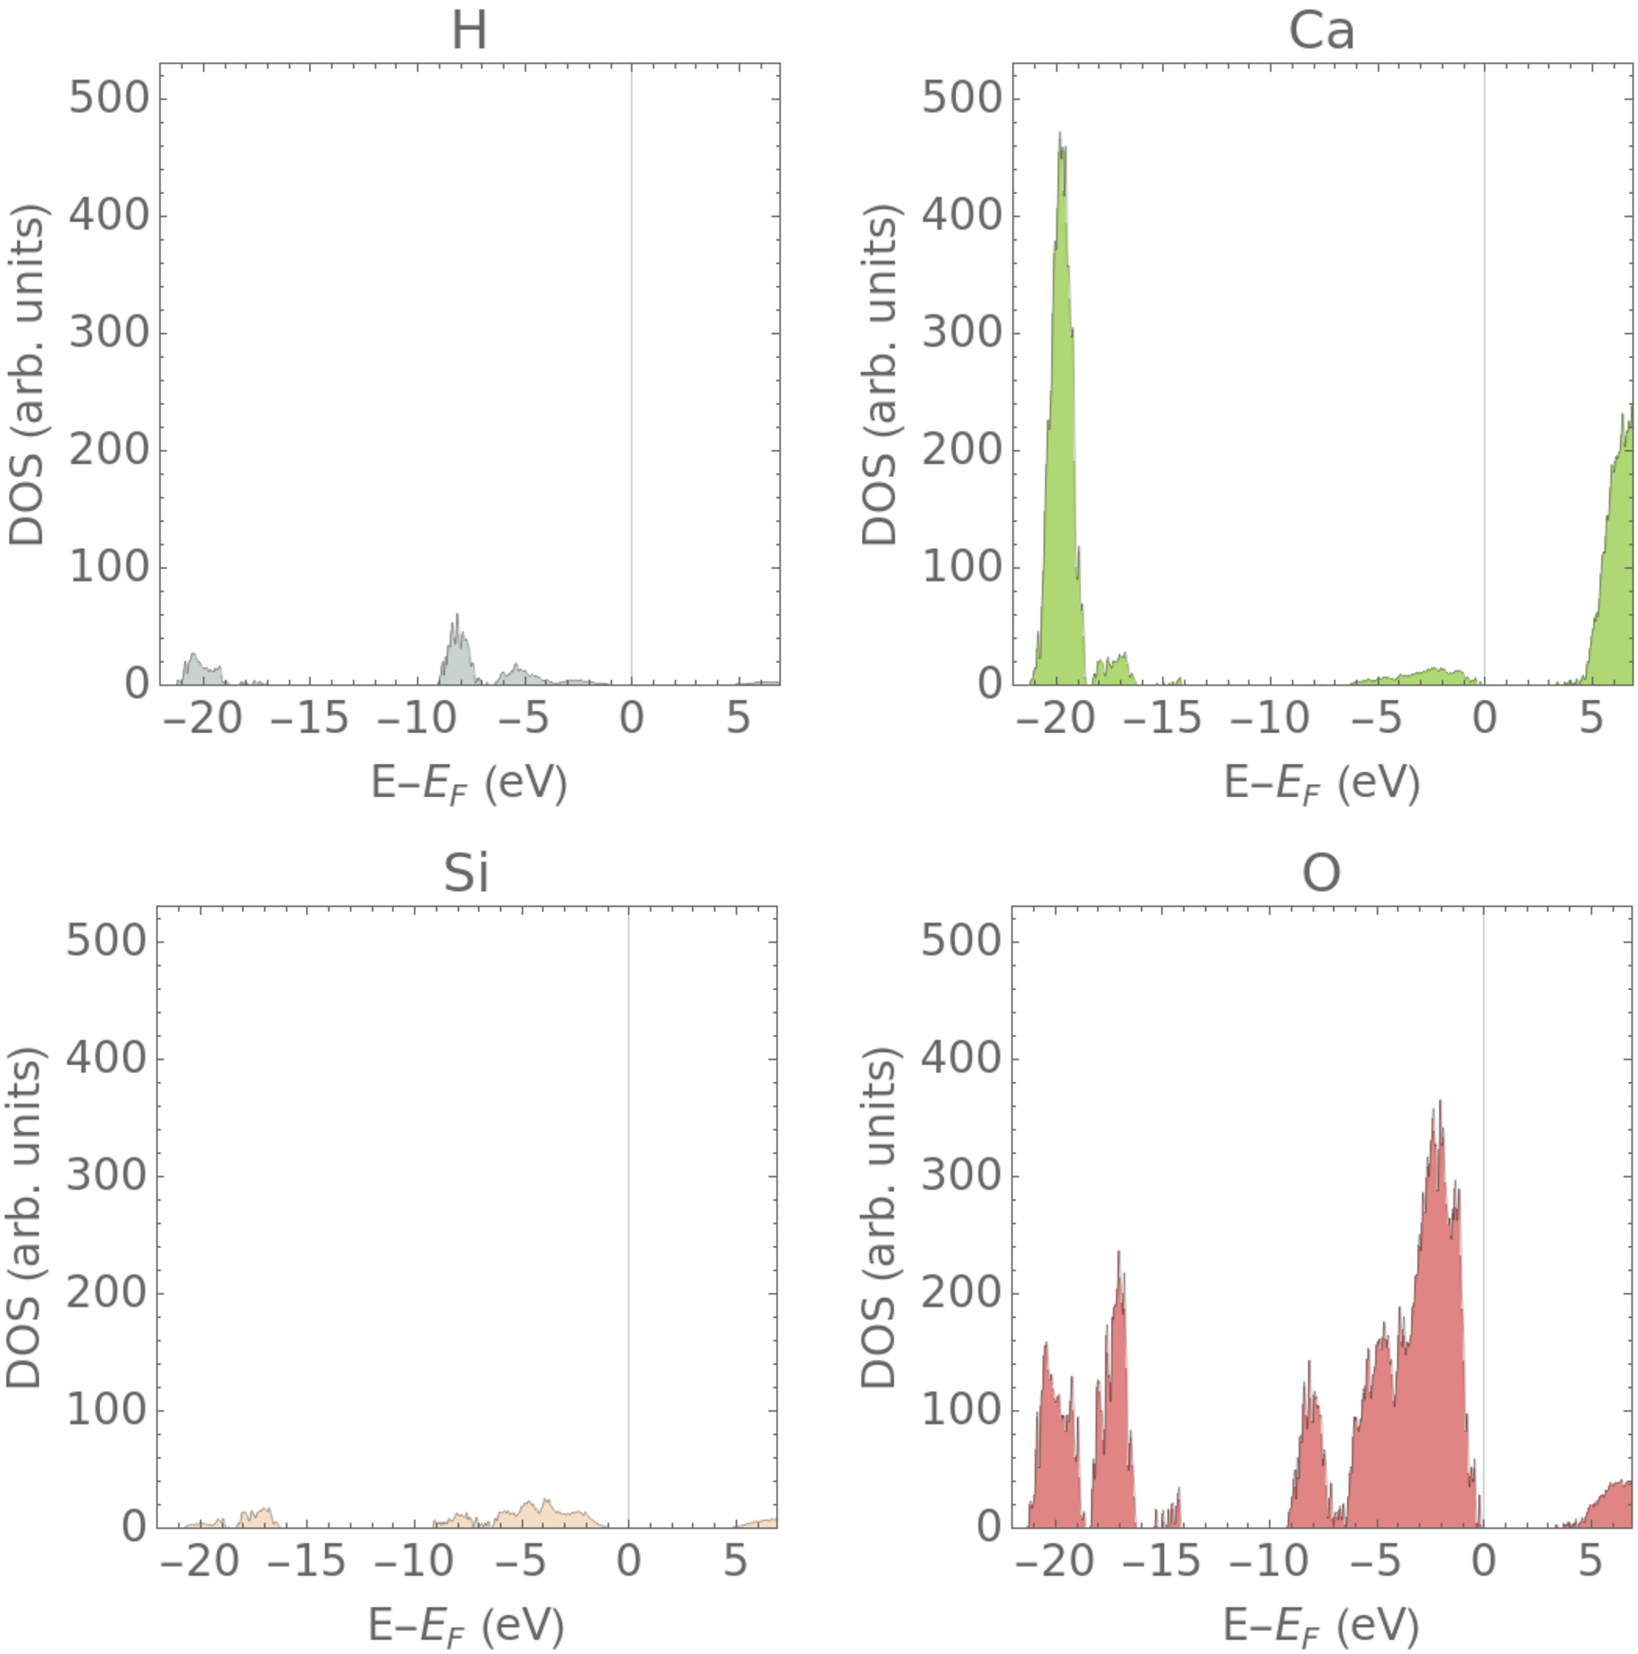
\includegraphics[width=0.8\textwidth]{PDOS.pdf}
    \caption{
        Here a caption 
    }
    \label{fig:pdos-all}
\end{figure}

%%\chapter{Appendix A} % Main appendix title
\appendix
\chapter{Computational Parameters} % Main appendix title
\label{AppendixB} % For referencing this appendix elsewhere, use \ref{AppendixA}


\begin{figure}[h]
    \centering
    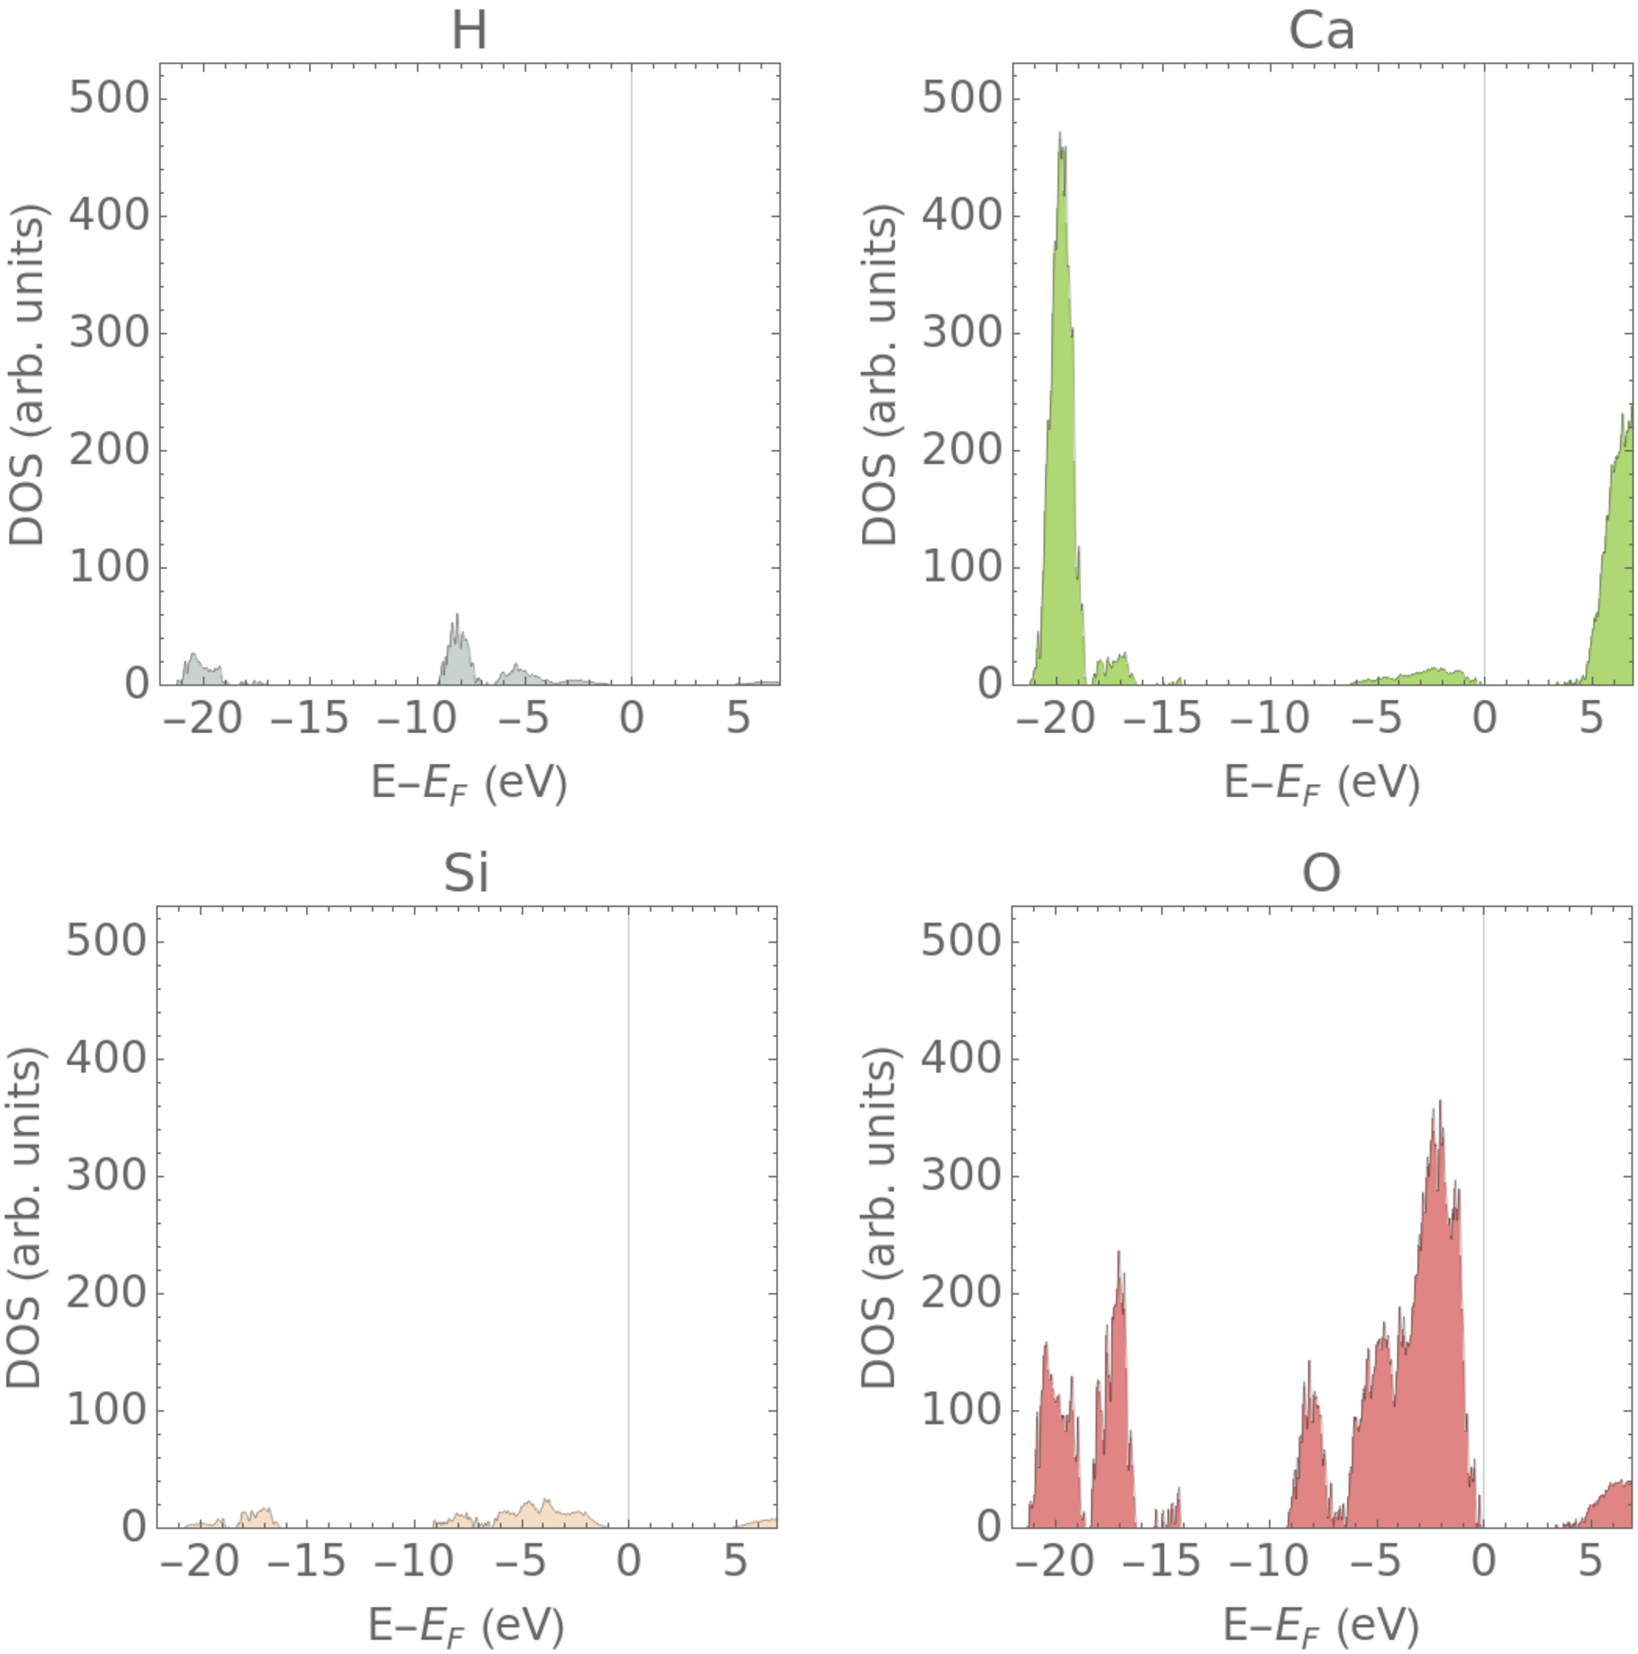
\includegraphics[width=0.8\textwidth]{PDOS.pdf}
    \caption{
        Here a caption 
    }
    \label{fig:pdos-all}
\end{figure}


%\input{Appendices/AppendixC}

\addtocontents{toc}{\vspace{2em}} % Add a gap in the Contents, for aesthetics

\backmatter

%-------------------------------------------------------------------------------
%	BIBLIOGRAPHY
%-------------------------------------------------------------------------------

\label{Bibliography}

\lhead{\emph{Bibliography}} % Change the page header to say "Bibliography"

\printbibliography

\end{document}
